% Complete extended iConference source. Requires the accompanying Font/ and Images/ folders.
% Compile with XeLaTeX, Biber, then XeLaTeX twice.
\begin{filecontents*}[overwrite]{iconference_embedded_references.bib}
% Bibliography checked 2026-09-05. No unverified DOI is retained.

@article{alcacer2006,
  author = {Alc{\'{a}}cer, Juan and Gittelman, Michelle},
  title = {Patent citations as a measure of knowledge flows: The influence of examiner citations},
  year = {2006},
  journal = {Review of Economics and Statistics},
  volume = {88},
  number = {4},
  pages = {774--779},
  doi = {10.1162/rest.88.4.774},
  url = {https://doi.org/10.1162/rest.88.4.774}
}

@article{benjamini1995,
  author = {Benjamini, Yoav and Hochberg, Yosef},
  title = {Controlling the false discovery rate: A practical and powerful approach to multiple testing},
  year = {1995},
  journal = {Journal of the Royal Statistical Society Series B: Statistical Methodology},
  volume = {57},
  number = {1},
  pages = {289--300},
  doi = {10.1111/j.2517-6161.1995.tb02031.x},
  url = {https://doi.org/10.1111/j.2517-6161.1995.tb02031.x}
}

@article{boccaletti2014,
  author = {Boccaletti, S. and Bianconi, G. and Criado, R. and del Genio, C.I. and G{\'{o}}mez-Garde{\~{n}}es, J. and Romance, M. and Sendi{\~{n}}a-Nadal, I. and Wang, Z. and Zanin, M.},
  title = {The structure and dynamics of multilayer networks},
  year = {2014},
  journal = {Physics Reports},
  volume = {544},
  number = {1},
  pages = {1--122},
  doi = {10.1016/j.physrep.2014.07.001},
  url = {https://doi.org/10.1016/j.physrep.2014.07.001}
}

@article{borner2003,
  author = {B{\"{o}}rner, Katy and Chen, Chaomei and Boyack, Kevin W.},
  title = {Visualizing knowledge domains},
  year = {2003},
  journal = {Annual Review of Information Science and Technology},
  volume = {37},
  number = {1},
  pages = {179--255},
  doi = {10.1002/aris.1440370106},
  url = {https://doi.org/10.1002/aris.1440370106}
}

@article{chen2006,
  author = {Chen, Chaomei},
  title = {{CiteSpace II}: Detecting and visualizing emerging trends and transient patterns in scientific literature},
  year = {2006},
  journal = {Journal of the American Society for Information Science and Technology},
  volume = {57},
  number = {3},
  pages = {359--377},
  doi = {10.1002/asi.20317},
  url = {https://doi.org/10.1002/asi.20317}
}

@article{cohen1960,
  author = {Cohen, Jacob},
  title = {A coefficient of agreement for nominal scales},
  year = {1960},
  journal = {Educational and Psychological Measurement},
  volume = {20},
  number = {1},
  pages = {37--46},
  doi = {10.1177/001316446002000104},
  url = {https://doi.org/10.1177/001316446002000104}
}

@article{cohen1990,
  author = {Cohen, Wesley M. and Levinthal, Daniel A.},
  title = {Absorptive capacity: A new perspective on learning and innovation},
  year = {1990},
  journal = {Administrative Science Quarterly},
  volume = {35},
  number = {1},
  pages = {128--152},
  doi = {10.2307/2393553},
  url = {https://doi.org/10.2307/2393553}
}

@article{dosi1982,
  author = {Dosi, Giovanni},
  title = {Technological paradigms and technological trajectories},
  year = {1982},
  journal = {Research Policy},
  volume = {11},
  number = {3},
  pages = {147--162},
  doi = {10.1016/0048-7333(82)90016-6},
  url = {https://doi.org/10.1016/0048-7333(82)90016-6}
}

@article{efron1979,
  author = {Efron, B.},
  title = {Bootstrap methods: Another look at the jackknife},
  year = {1979},
  journal = {The Annals of Statistics},
  volume = {7},
  number = {1},
  pages = {1--26},
  doi = {10.1214/aos/1176344552},
  url = {https://doi.org/10.1214/aos/1176344552}
}

@article{fleming2001,
  author = {Fleming, Lee},
  title = {Recombinant uncertainty in technological search},
  year = {2001},
  journal = {Management Science},
  volume = {47},
  number = {1},
  pages = {117--132},
  doi = {10.1287/mnsc.47.1.117.10671},
  url = {https://doi.org/10.1287/mnsc.47.1.117.10671}
}

@article{fleming2004,
  author = {Fleming, Lee and Sorenson, Olav},
  title = {Science as a map in technological search},
  year = {2004},
  journal = {Strategic Management Journal},
  volume = {25},
  number = {8-9},
  pages = {909--928},
  doi = {10.1002/smj.384},
  url = {https://doi.org/10.1002/smj.384}
}

@article{fraley2002,
  author = {Fraley, Chris and Raftery, Adrian E},
  title = {Model-based clustering, discriminant analysis, and density estimation},
  year = {2002},
  journal = {Journal of the American Statistical Association},
  volume = {97},
  number = {458},
  pages = {611--631},
  doi = {10.1198/016214502760047131},
  url = {https://doi.org/10.1198/016214502760047131}
}

@article{funk2017,
  author = {Funk, Russell J. and Owen-Smith, Jason},
  title = {A dynamic network measure of technological change},
  year = {2017},
  journal = {Management Science},
  volume = {63},
  number = {3},
  pages = {791--817},
  doi = {10.1287/mnsc.2015.2366},
  url = {https://doi.org/10.1287/mnsc.2015.2366}
}

@article{griliches1990,
  author = {Griliches, Zvi},
  title = {Patent statistics as economic indicators: A survey},
  journal = {Journal of Economic Literature},
  year = {1990},
  volume = {28},
  number = {4},
  pages = {1661--1707},
  url = {https://www.jstor.org/stable/2727442}
}

@article{hall2005,
  author = {Hall, Bronwyn H. and Jaffe, Adam and Trajtenberg, Manuel},
  title = {Market value and patent citations},
  journal = {The RAND Journal of Economics},
  year = {2005},
  volume = {36},
  number = {1},
  pages = {16--38},
  url = {https://www.jstor.org/stable/1593752}
}

@article{hennig2007,
  author = {Hennig, Christian},
  title = {Cluster-wise assessment of cluster stability},
  year = {2007},
  journal = {Computational Statistics \& Data Analysis},
  volume = {52},
  number = {1},
  pages = {258--271},
  doi = {10.1016/j.csda.2006.11.025},
  url = {https://doi.org/10.1016/j.csda.2006.11.025}
}

@article{hicks2015,
  author = {Hicks, Diana and Wouters, Paul and Waltman, Ludo and de Rijcke, Sarah and Rafols, Ismael},
  title = {Bibliometrics: The {Leiden} manifesto for research metrics},
  year = {2015},
  journal = {Nature},
  volume = {520},
  number = {7548},
  pages = {429--431},
  doi = {10.1038/520429a},
  url = {https://doi.org/10.1038/520429a}
}

@article{huang2019,
  author = {Huang, Yong and Bu, Yi and Ding, Ying and Lu, Wei},
  title = {From zero to one: A perspective on citing},
  year = {2019},
  journal = {Journal of the Association for Information Science and Technology},
  volume = {70},
  number = {10},
  pages = {1098--1107},
  doi = {10.1002/asi.24177},
  url = {https://doi.org/10.1002/asi.24177}
}

@article{hubert1985,
  author = {Hubert, Lawrence and Arabie, Phipps},
  title = {Comparing partitions},
  year = {1985},
  journal = {Journal of Classification},
  volume = {2},
  number = {1},
  pages = {193--218},
  doi = {10.1007/bf01908075},
  url = {https://doi.org/10.1007/bf01908075}
}

@article{jaffe1993,
  author = {Jaffe, A. B. and Trajtenberg, M. and Henderson, R.},
  title = {Geographic localization of knowledge spillovers as evidenced by patent citations},
  year = {1993},
  journal = {The Quarterly Journal of Economics},
  volume = {108},
  number = {3},
  pages = {577--598},
  doi = {10.2307/2118401},
  url = {https://doi.org/10.2307/2118401}
}

@article{katila2002,
  author = {Katila, R. and Ahuja, G.},
  title = {Something old, something new: A longitudinal study of search behavior and new product introduction},
  year = {2002},
  journal = {Academy of Management Journal},
  volume = {45},
  number = {6},
  pages = {1183--1194},
  doi = {10.2307/3069433},
  url = {https://doi.org/10.2307/3069433}
}

@article{kay2014,
  author = {Kay, Luciano and Newman, Nils and Youtie, Jan and Porter, Alan L. and Rafols, Ismael},
  title = {Patent overlay mapping: Visualizing technological distance},
  year = {2014},
  journal = {Journal of the Association for Information Science and Technology},
  volume = {65},
  number = {12},
  pages = {2432--2443},
  doi = {10.1002/asi.23146},
  url = {https://doi.org/10.1002/asi.23146}
}

@article{kelly2021,
  author = {Kelly, Bryan and Papanikolaou, Dimitris and Seru, Amit and Taddy, Matt},
  title = {Measuring technological innovation over the long run},
  year = {2021},
  journal = {American Economic Review: Insights},
  volume = {3},
  number = {3},
  pages = {303--320},
  doi = {10.1257/aeri.20190499},
  url = {https://doi.org/10.1257/aeri.20190499}
}

@article{kessler1963,
  author = {Kessler, M. M.},
  title = {Bibliographic coupling between scientific papers},
  year = {1963},
  journal = {American Documentation},
  volume = {14},
  number = {1},
  pages = {10--25},
  doi = {10.1002/asi.5090140103},
  url = {https://doi.org/10.1002/asi.5090140103}
}

@article{kivela2014,
  author = {Kivela, M. and Arenas, A. and Barthelemy, M. and Gleeson, J. P. and Moreno, Y. and Porter, M. A.},
  title = {Multilayer networks},
  year = {2014},
  journal = {Journal of Complex Networks},
  volume = {2},
  number = {3},
  pages = {203--271},
  doi = {10.1093/comnet/cnu016},
  url = {https://doi.org/10.1093/comnet/cnu016}
}

@article{kogler2013,
  author = {Kogler, Dieter F. and Rigby, David L. and Tucker, Isaac},
  title = {Mapping knowledge space and technological relatedness in {US} cities},
  year = {2013},
  journal = {European Planning Studies},
  volume = {21},
  number = {9},
  pages = {1374--1391},
  doi = {10.1080/09654313.2012.755832},
  url = {https://doi.org/10.1080/09654313.2012.755832}
}

@article{leydesdorff2008,
  author = {Leydesdorff, Loet},
  title = {Patent classifications as indicators of intellectual organization},
  year = {2008},
  journal = {Journal of the American Society for Information Science and Technology},
  volume = {59},
  number = {10},
  pages = {1582--1597},
  doi = {10.1002/asi.20814},
  url = {https://doi.org/10.1002/asi.20814}
}

@article{leydesdorff2014,
  author = {Leydesdorff, Loet and Kushnir, Duncan and Rafols, Ismael},
  title = {Interactive overlay maps for {US} patent ({USPTO}) data based on {International Patent Classification} ({IPC})},
  year = {2014},
  journal = {Scientometrics},
  volume = {98},
  number = {3},
  pages = {1583--1599},
  doi = {10.1007/s11192-012-0923-2},
  url = {https://doi.org/10.1007/s11192-012-0923-2}
}

@article{lin1991,
  author = {Lin, J.},
  title = {Divergence measures based on the {Shannon} entropy},
  year = {1991},
  journal = {IEEE Transactions on Information Theory},
  volume = {37},
  number = {1},
  pages = {145--151},
  doi = {10.1109/18.61115},
  url = {https://doi.org/10.1109/18.61115}
}

@article{march1991,
  author = {March, James G.},
  title = {Exploration and exploitation in organizational learning},
  year = {1991},
  journal = {Organization Science},
  volume = {2},
  number = {1},
  pages = {71--87},
  doi = {10.1287/orsc.2.1.71},
  url = {https://doi.org/10.1287/orsc.2.1.71}
}

@article{mucha2010,
  author = {Mucha, Peter J. and Richardson, Thomas and Macon, Kevin and Porter, Mason A. and Onnela, Jukka-Pekka},
  title = {Community structure in time-dependent, multiscale, and multiplex networks},
  year = {2010},
  journal = {Science},
  volume = {328},
  number = {5980},
  pages = {876--878},
  doi = {10.1126/science.1184819},
  url = {https://doi.org/10.1126/science.1184819}
}

@incollection{nagaoka2010,
  author = {Nagaoka, Sadao and Motohashi, Kazuyuki and Goto, Akira},
  title = {Patent statistics as an innovation indicator},
  year = {2010},
  booktitle = {Handbook of the Economics of Innovation},
  volume = {2},
  publisher = {Elsevier},
  pages = {1083--1127},
  doi = {10.1016/s0169-7218(10)02009-5},
  url = {https://doi.org/10.1016/s0169-7218(10)02009-5}
}

@article{palla2007,
  author = {Palla, Gergely and Barab{\'{a}}si, Albert-L{\'{a}}szl{\'{o}} and Vicsek, Tam{\'{a}}s},
  title = {Quantifying social group evolution},
  year = {2007},
  journal = {Nature},
  volume = {446},
  number = {7136},
  pages = {664--667},
  doi = {10.1038/nature05670},
  url = {https://doi.org/10.1038/nature05670}
}

@article{porter2009,
  author = {Porter, Alan L. and Rafols, Ismael},
  title = {Is science becoming more interdisciplinary? measuring and mapping six research fields over time},
  year = {2009},
  journal = {Scientometrics},
  volume = {81},
  number = {3},
  pages = {719--745},
  doi = {10.1007/s11192-008-2197-2},
  url = {https://doi.org/10.1007/s11192-008-2197-2}
}

@article{price1965,
  author = {Price, Derek J. de Solla},
  title = {Networks of scientific papers},
  year = {1965},
  journal = {Science},
  volume = {149},
  number = {3683},
  pages = {510--515},
  doi = {10.1126/science.149.3683.510},
  url = {https://doi.org/10.1126/science.149.3683.510}
}

@article{rafols2010,
  author = {Rafols, Ismael and Porter, Alan L. and Leydesdorff, Loet},
  title = {Science overlay maps: A new tool for research policy and library management},
  year = {2010},
  journal = {Journal of the American Society for Information Science and Technology},
  volume = {61},
  number = {9},
  pages = {1871--1887},
  doi = {10.1002/asi.21368},
  url = {https://doi.org/10.1002/asi.21368}
}

@inproceedings{reimers2019,
  author = {Reimers, Nils and Gurevych, Iryna},
  title = {{Sentence-BERT}: Sentence embeddings using siamese {BERT}-networks},
  year = {2019},
  booktitle = {Proceedings of the 2019 Conference on Empirical Methods in Natural Language Processing and the 9th International Joint Conference on Natural Language Processing (EMNLP-IJCNLP)},
  publisher = {Association for Computational Linguistics},
  pages = {3980--3990},
  doi = {10.18653/v1/d19-1410},
  url = {https://doi.org/10.18653/v1/d19-1410}
}

@article{rigby2015,
  author = {Rigby, David L.},
  title = {Technological relatedness and knowledge space: Entry and exit of {US} cities from patent classes},
  year = {2015},
  journal = {Regional Studies},
  volume = {49},
  number = {11},
  pages = {1922--1937},
  doi = {10.1080/00343404.2013.854878},
  url = {https://doi.org/10.1080/00343404.2013.854878}
}

@article{rotolo2015,
  author = {Rotolo, Daniele and Hicks, Diana and Martin, Ben R.},
  title = {What is an emerging technology?},
  year = {2015},
  journal = {Research Policy},
  volume = {44},
  number = {10},
  pages = {1827--1843},
  doi = {10.1016/j.respol.2015.06.006},
  url = {https://doi.org/10.1016/j.respol.2015.06.006}
}

@article{rousseeuw1987,
  author = {Rousseeuw, Peter J.},
  title = {Silhouettes: A graphical aid to the interpretation and validation of cluster analysis},
  year = {1987},
  journal = {Journal of Computational and Applied Mathematics},
  volume = {20},
  pages = {53--65},
  doi = {10.1016/0377-0427(87)90125-7},
  url = {https://doi.org/10.1016/0377-0427(87)90125-7}
}

@article{sarica2020,
  author = {Sarica, Serhad and Luo, Jianxi and Wood, Kristin L.},
  title = {{TechNet}: Technology semantic network based on patent data},
  year = {2020},
  journal = {Expert Systems with Applications},
  volume = {142},
  pages = {112995},
  doi = {10.1016/j.eswa.2019.112995},
  url = {https://doi.org/10.1016/j.eswa.2019.112995}
}

@article{schwarz1978,
  author = {Schwarz, Gideon},
  title = {Estimating the dimension of a model},
  year = {1978},
  journal = {The Annals of Statistics},
  volume = {6},
  number = {2},
  pages = {461--464},
  doi = {10.1214/aos/1176344136},
  url = {https://doi.org/10.1214/aos/1176344136}
}

@article{scrucca2016,
  author = {Scrucca, Luca and Fop, Michael and Murphy, T.,Brendan and Raftery, Adrian,E.},
  title = {{mclust} 5: Clustering, classification and density estimation using {Gaussian} finite mixture models},
  year = {2016},
  journal = {The R Journal},
  volume = {8},
  number = {1},
  pages = {289--317},
  doi = {10.32614/rj-2016-021},
  url = {https://doi.org/10.32614/rj-2016-021}
}

@article{shannon1948,
  author = {Shannon, C. E.},
  title = {A mathematical theory of communication},
  year = {1948},
  journal = {Bell System Technical Journal},
  volume = {27},
  number = {3},
  pages = {379--423},
  doi = {10.1002/j.1538-7305.1948.tb01338.x},
  url = {https://doi.org/10.1002/j.1538-7305.1948.tb01338.x}
}

@article{small1973,
  author = {Small, Henry},
  title = {Co-citation in the scientific literature: A new measure of the relationship between two documents},
  year = {1973},
  journal = {Journal of the American Society for Information Science},
  volume = {24},
  number = {4},
  pages = {265--269},
  doi = {10.1002/asi.4630240406},
  url = {https://doi.org/10.1002/asi.4630240406}
}

@article{small2014,
  author = {Small, Henry and Boyack, Kevin W. and Klavans, Richard},
  title = {Identifying emerging topics in science and technology},
  year = {2014},
  journal = {Research Policy},
  volume = {43},
  number = {8},
  pages = {1450--1467},
  doi = {10.1016/j.respol.2014.02.005},
  url = {https://doi.org/10.1016/j.respol.2014.02.005}
}

@article{stirling2007,
  author = {Stirling, Andy},
  title = {A general framework for analysing diversity in science, technology and society},
  year = {2007},
  journal = {Journal of The Royal Society Interface},
  volume = {4},
  number = {15},
  pages = {707--719},
  doi = {10.1098/rsif.2007.0213},
  url = {https://doi.org/10.1098/rsif.2007.0213}
}

@article{thompson2005,
  author = {Thompson, Peter and Fox-Kean, Melanie},
  title = {Patent citations and the geography of knowledge spillovers: A reassessment},
  year = {2005},
  journal = {American Economic Review},
  volume = {95},
  number = {1},
  pages = {450--460},
  doi = {10.1257/0002828053828509},
  url = {https://doi.org/10.1257/0002828053828509}
}

@article{traag2019,
  author = {Traag, V. A. and Waltman, L. and van Eck, N. J.},
  title = {From {Louvain} to {Leiden}: Guaranteeing well-connected communities},
  year = {2019},
  journal = {Scientific Reports},
  volume = {9},
  number = {1},
  pages = {5233},
  doi = {10.1038/s41598-019-41695-z},
  url = {https://doi.org/10.1038/s41598-019-41695-z}
}

@article{trajtenberg1990,
  author = {Trajtenberg, Manuel},
  title = {A penny for your quotes: Patent citations and the value of innovations},
  year = {1990},
  journal = {The RAND Journal of Economics},
  volume = {21},
  number = {1},
  pages = {172--187},
  doi = {10.2307/2555502},
  url = {https://doi.org/10.2307/2555502}
}

@article{uzzi2013,
  author = {Uzzi, Brian and Mukherjee, Satyam and Stringer, Michael and Jones, Ben},
  title = {Atypical combinations and scientific impact},
  year = {2013},
  journal = {Science},
  volume = {342},
  number = {6157},
  pages = {468--472},
  doi = {10.1126/science.1240474},
  url = {https://doi.org/10.1126/science.1240474}
}

@article{vaneck2010,
  author = {van Eck, Nees Jan and Waltman, Ludo},
  title = {Software survey: {VOSviewer}, a computer program for bibliometric mapping},
  year = {2010},
  journal = {Scientometrics},
  volume = {84},
  number = {2},
  pages = {523--538},
  doi = {10.1007/s11192-009-0146-3},
  url = {https://doi.org/10.1007/s11192-009-0146-3}
}

@article{verhoeven2016,
  author = {Verhoeven, Dennis and Bakker, Jurri{\"{e}}n and Veugelers, Reinhilde},
  title = {Measuring technological novelty with patent-based indicators},
  year = {2016},
  journal = {Research Policy},
  volume = {45},
  number = {3},
  pages = {707--723},
  doi = {10.1016/j.respol.2015.11.010},
  url = {https://doi.org/10.1016/j.respol.2015.11.010}
}

@article{wang2017,
  author = {Wang, Jian and Veugelers, Reinhilde and Stephan, Paula},
  title = {Bias against novelty in science: A cautionary tale for users of bibliometric indicators},
  year = {2017},
  journal = {Research Policy},
  volume = {46},
  number = {8},
  pages = {1416--1436},
  doi = {10.1016/j.respol.2017.06.006},
  url = {https://doi.org/10.1016/j.respol.2017.06.006}
}

@article{whalen2020,
  author = {Whalen, Ryan and Lungeanu, Alina and DeChurch, Leslie and Contractor, Noshir},
  title = {Patent similarity data and innovation metrics},
  year = {2020},
  journal = {Journal of Empirical Legal Studies},
  volume = {17},
  number = {3},
  pages = {615--639},
  doi = {10.1111/jels.12261},
  url = {https://doi.org/10.1111/jels.12261}
}

@article{wilkinson2016,
  author = {Wilkinson, Mark D. and Dumontier, Michel and Aalbersberg, IJsbrand Jan and Appleton, Gabrielle and Axton, Myles and Baak, Arie and Blomberg, Niklas and Boiten, Jan-Willem and da Silva Santos, Luiz Bonino and Bourne, Philip E. and Bouwman, Jildau and Brookes, Anthony J. and Clark, Tim and Crosas, Merc{\`{e}} and Dillo, Ingrid and Dumon, Olivier and Edmunds, Scott and Evelo, Chris T. and Finkers, Richard and Gonzalez-Beltran, Alejandra and Gray, Alasdair J.G. and Groth, Paul and Goble, Carole and Grethe, Jeffrey S. and Heringa, Jaap and 't Hoen, Peter A.C and Hooft, Rob and Kuhn, Tobias and Kok, Ruben and Kok, Joost and Lusher, Scott J. and Martone, Maryann E. and Mons, Albert and Packer, Abel L. and Persson, Bengt and Rocca-Serra, Philippe and Roos, Marco and van Schaik, Rene and Sansone, Susanna-Assunta and Schultes, Erik and Sengstag, Thierry and Slater, Ted and Strawn, George and Swertz, Morris A. and Thompson, Mark and van der Lei, Johan and van Mulligen, Erik and Velterop, Jan and Waagmeester, Andra and Wittenburg, Peter and Wolstencroft, Katherine and Zhao, Jun and Mons, Barend},
  title = {The {FAIR} guiding principles for scientific data management and stewardship},
  year = {2016},
  journal = {Scientific Data},
  volume = {3},
  number = {1},
  pages = {160018},
  doi = {10.1038/sdata.2016.18},
  url = {https://doi.org/10.1038/sdata.2016.18}
}

@article{yan2017,
  author = {Yan, Bowen and Luo, Jianxi},
  title = {Measuring technological distance for patent mapping},
  year = {2017},
  journal = {Journal of the Association for Information Science and Technology},
  volume = {68},
  number = {2},
  pages = {423--437},
  doi = {10.1002/asi.23664},
  url = {https://doi.org/10.1002/asi.23664}
}

@article{youn2015,
  author = {Youn, Hyejin and Strumsky, Deborah and Bettencourt, Luis M. A. and Lobo, Jos{\'{e}}},
  title = {Invention as a combinatorial process: Evidence from {US} patents},
  year = {2015},
  journal = {Journal of The Royal Society Interface},
  volume = {12},
  number = {106},
  pages = {20150272},
  doi = {10.1098/rsif.2015.0272},
  url = {https://doi.org/10.1098/rsif.2015.0272}
}

\end{filecontents*}
\documentclass[12pt]{article}
\usepackage[a4paper,margin=1in,bottom=35mm]{geometry}
\usepackage{titlesec}
\usepackage[table]{xcolor}
\definecolor{darkforestgreen}{RGB}{1,68,42}
\titleformat{\section}[block]{\normalfont\bfseries\Large\color{darkforestgreen}}{\thesection.}{1em}{}
\titleformat{\subsection}[block]{\normalfont\bfseries\large\color{darkforestgreen}}{\thesubsection.}{1em}{}
\titleformat{\subsubsection}[block]{\normalfont\bfseries\normalsize\color{darkforestgreen}}{\thesubsubsection.}{1em}{}
\usepackage{graphicx,caption,array,tabularx,longtable,booktabs,multirow}
\usepackage{ragged2e,changepage,quoting,enumitem,setspace}
\usepackage{amsmath,amssymb,mathtools}
\usepackage{fontspec}
\setmainfont{Lora-Regular.ttf}[Path=Font/,BoldFont=Lora-SemiBold.ttf,
 ItalicFont=Lora-Italic.ttf,BoldItalicFont=Lora-SemiBoldItalic.ttf]
\usepackage{tikz}
\usetikzlibrary{arrows.meta,positioning,fit,calc,backgrounds}
\usepackage{float,placeins}
\usepackage{xurl}
\usepackage[colorlinks=true,linkcolor=blue,citecolor=black,urlcolor=blue,
 pdftitle={Mapping Technological Knowledge Evolution in Chinese Universities},pdfauthor={}]{hyperref}
% Compatibility for older LaTeX kernels without PDF-metadata tagging.
\providecommand\IfDocumentMetadataT[1]{}
\providecommand\IfDocumentMetadataF[1]{#1}
\providecommand\IfDocumentMetadataTF[2]{#2}
\usepackage[backend=biber,style=apa,natbib=true]{biblatex}
\addbibresource{iconference_embedded_references.bib}
\AtBeginEnvironment{longtable}{\fontsize{9}{11}\selectfont}
\AtBeginBibliography{\setlength{\itemsep}{1\baselineskip}}
\usepackage{fancyhdr}
\pagestyle{fancy}\fancyhf{}
\renewcommand{\headrulewidth}{0pt}\renewcommand{\footrulewidth}{0pt}
\fancyfoot[C]{\vspace{0.5em}Information Research, Vol. ?? No. ? (20??)\\
 \rule{0.65\linewidth}{0.4pt}\\\thepage}
\setcounter{secnumdepth}{0}
\setlength{\parindent}{0pt}
\setlength{\emergencystretch}{2em}
\newenvironment{blockquote}{\vspace{1em}\begin{adjustwidth}{5em}{0em}\justifying\setlength{\parindent}{0pt}\normalsize}{\end{adjustwidth}\vspace{1em}}
\usepackage{titling}
\title{\textcolor{darkforestgreen}{Mapping Technological Knowledge Evolution in Chinese Universities}}
\newenvironment{structuredabstract}{\section*{Abstract}}{}
\DeclareCaptionFont{nine}{\fontsize{9}{11}\selectfont}
\captionsetup{font=nine,labelfont=bf,labelsep=period,justification=centering}
\newcolumntype{Y}{>{\raggedright\arraybackslash}X}
\newcolumntype{P}[1]{>{\raggedright\arraybackslash}p{#1}}
\newcommand{\TBD}{\textsf{TBD}}
\newcommand{\pending}[1]{\textsf{[Pending: #1]}}
\newcommand{\ind}{\mathbb{I}}
\newcommand{\E}{\mathbb{E}}
\newcommand{\R}{\mathbb{R}}
\newcommand{\KL}{D_{\mathrm{KL}}}
\newcommand{\JSD}{\operatorname{JSD}}
\newcommand{\NA}{\textsf{NA}}
\newcommand{\clip}{\operatorname{clip}}
\newcommand{\dd}{\mathrm{d}}
\newcommand{\figpanel}[3]{\begin{minipage}[t]{#1}\raggedright\small\textbf{#2}\par\medskip
 \fbox{\begin{minipage}{\dimexpr\linewidth-2\fboxsep-2\fboxrule}\centering\small
 \vspace{0.6em}#3\par\vspace{0.6em}\end{minipage}}\end{minipage}}
\tikzset{box/.style={draw=black,rounded corners=3pt,fill=white,align=center,
 inner sep=7pt,font=\small},arr/.style={-{Latex[length=2mm]},thick},
 note/.style={font=\footnotesize,align=center}}

\begin{document}
\setlength{\parindent}{0pt}
\begin{center}

\includegraphics[width=0.2\textwidth]{Images/IR_Bild.png}
\\\vspace{1em}
{\normalsize Information Research - Vol. ?? No. ? (20??)\par}
\vspace{1em}
{\LARGE\bfseries\thetitle\par}
\end{center}
\begin{center}
DOI: \emph{leave as is, will be created by the journal}\\\vspace{1em}
\end{center}
\begin{adjustwidth}{1.2cm}{1.2cm}
\begin{structuredabstract}
\medskip\textbf{Introduction.} Patent indicators describe inventive output, whereas understanding knowledge evolution also requires tracing sources, technical combinations, emerging directions, and subsequent use. This study develops a framework for Chinese universities.

\medskip\textbf{Method.} Dated patent objects connect classifications, text, organizations, and citations through three complementary network layers. Four process dimensions measure acquisition, recombination, recognized emergence, and diffusion. Transformation is assessed independently as sustained structural change.

\medskip\textbf{Analysis.} Gaussian mixture models summarize university-period profiles; transition matrices describe state sequences. Fixed citation horizons, university-level resampling, blinded case assessment, and time-separated validation specify how the framework will be evaluated.

\medskip\textbf{Results.} This draft provides operational definitions and an empirical reporting design. The source database has not been supplied, so distributions, state counts, and transition probabilities remain uncomputed. Maintenance, expansion, recombination, and transformation are proposed trajectory interpretations rather than established findings.

\medskip\textbf{Conclusion.} The framework connects knowledge organization and patent mapping to longitudinal institutional analysis. Its empirical usefulness depends on whether relational distinctions survive controls for patent volume, technological field, coverage, and observation time.
\end{structuredabstract}
\end{adjustwidth}

\noindent\emph{Complete extended working version; empirical analysis pending.}
\section{Introduction}\label{sec:introduction}
Universities contribute to technological development through inventions that draw
on established knowledge, combine technical components, and create opportunities
for further work. Patent documents provide a distinctive information resource for
studying these processes because they connect technical descriptions to formal
classifications, prior-art references, organizational identities, and dates. The
analytical challenge is to turn these heterogeneous records into an account of how
knowledge structures change. Counting documents alone cannot establish whether an
institution is deepening an existing specialization, entering adjacent technical
areas, combining previously disconnected elements, or sustaining a new direction.

Patent counts and citations nevertheless have legitimate uses. They support
measurement of inventive activity and subsequent technological attention, subject
to differences in patenting propensity, sector, jurisdiction, and citation practice
\citep{griliches1990,nagaoka2010,hall2005}. Citation-based indicators can also be
associated with the value of inventions \citep{trajtenberg1990}. The issue addressed
here is therefore an additional explanatory requirement: an evolutionary analysis
needs to distinguish the processes generating apparently similar output profiles.
Two universities with comparable patent volumes may have different knowledge
sources, different combinations of technical elements, and different patterns of
subsequent use. Those differences are obscured when all dimensions are reduced to
a single performance score.

Information science provides a foundation for examining this problem. Bibliographic
coupling, co-citation analysis, and knowledge-domain visualization relate documents
through their intellectual connections \citep{kessler1963,small1973,price1965,borner2003}.
Science mapping makes these relations visible across fields and over time
\citep{chen2006,vaneck2010,rafols2010}. Patent mapping already extends this tradition
to technological information, including classification-based overlays and measures
of technological distance \citep{kay2014,leydesdorff2014,yan2017}. Accordingly, the
present study does not claim to introduce patents into science mapping. It asks how
existing mapping capabilities can be organized into a coherent, temporally explicit
account of institution-level knowledge evolution.

Three difficulties motivate the framework. First, relations derived from
classification, text, and citations have different meanings. Shared classifications
indicate technical proximity, similar language indicates semantic proximity, and a
citation records a documented connection to prior art. Treating them as interchangeable
links weakens interpretation. Second, evolutionary constructs operate on different
timescales. Recombination can be observed when a patent becomes public, whereas
recognition, diffusion, and sustained transformation require subsequent observations.
Ignoring that distinction can introduce future information into a supposedly early
indicator. Third, a cluster of universities at one time is not itself an evolutionary
trajectory. A trajectory requires an ordered sequence of observations and evidence
that changes exceed classification noise and fluctuations in patent volume.

Chinese university patent data provide the intended empirical setting. A broad
institutional population can support comparisons among different technological
portfolios without defining the sample through a ranking or restricting it to a
small group of highly visible institutions. However, the claim of comprehensive
coverage must be established against an explicit university roster and database
retrieval audit. University-held patents also delimit the observable knowledge
system: without external citing records, the analysis cannot describe economy-wide
diffusion. These boundaries form part of the research design rather than assumptions
to be hidden in the results.

The study addresses three connected research questions:
\begin{enumerate}[label=\textbf{RQ\arabic*.}]
\item How can acquisition, recombination, emergence, and diffusion be operationalized
from complementary patent relations while preserving their conceptual and temporal
differences?
\item What recurring university-period knowledge profiles and longitudinal trajectories
are supported by the observed data, and how much of their variation is explained by
patent volume and technological composition?
\item Which state transitions coincide with sustained structural transformation,
and do the resulting descriptions remain informative under alternative representations,
observation windows, and independent validation?
\end{enumerate}

The proposed contribution has three parts. The theoretical contribution is to
distinguish four observable process dimensions from transformation as a longitudinal
outcome. This makes it possible to ask whether acquisition and recombination are
followed by emergence and diffusion without presuming that every invention follows
one sequence. The methodological contribution is a common measurement architecture
that retains network-layer meaning, defines observation horizons, and connects
probabilistic states to directly measured structural change. The disciplinary
contribution is to connect knowledge organization with institutional trajectory
analysis: maps become evidence for tracing changing relations rather than only
visual summaries of a technological landscape. Empirical support for these
contributions must come from the tests below; heterogeneous trajectories cannot be
inferred from the framework alone.

\section{Related work}\label{sec:related}
\subsection{Patents as indicators and information objects}
Patent statistics are established indicators of inventive activity, but they are
selective records of knowledge production. Some inventions are not patented, patent
quality varies, and legal and organizational strategies influence observed records
\citep{griliches1990,nagaoka2010}. Citation counts supply additional information, but
their interpretation depends on who adds citations and how prior art is identified.
Examiner-generated references limit the use of citations as direct measures of
inventor learning \citep{alcacer2006}. Spatial spillover analyses similarly depend
on the construction of comparison groups and technological controls
\citep{jaffe1993,thompson2005}. These findings support a restrained interpretation:
patents document technical claims and relations, not the complete cognitive or
economic history of an invention.

An information-object perspective adds analytical structure to that restraint.
The same patent can be classified within a technical taxonomy, located in a semantic
space, connected to predecessors, and followed through later citations. These
representations answer different questions and can disagree. Classification
systems reflect organized technical categories \citep{leydesdorff2008}, while text
can identify similarities that are not well represented by a shared class
\citep{whalen2020,kelly2021,sarica2020}. The useful contribution of integration is
therefore traceable complementarity, rather than an unexamined composite measure.

\subsection{Science mapping and technological knowledge spaces}
Classical document-relation methods establish intellectual proximity through
shared references or shared citations \citep{kessler1963,small1973}. Later mapping
systems support the detection of research fronts and the visualization of domain
structure \citep{borner2003,chen2006,vaneck2010}. Overlay maps enable the comparison
of organizations against a common background rather than a separate layout for
each portfolio \citep{rafols2010}. Patent overlays and technological-distance
research adapt these ideas to invention records
\citep{kay2014,leydesdorff2014,yan2017}.

Relatedness studies further connect positions in technological space to subsequent
entry and exit \citep{kogler2013,rigby2015}. A map can thus support an evolutionary
question, but an observed shift in its layout is not sufficient evidence of
transformation. Layout algorithms, changing classification coverage, and changes
in sample size can also move points. This study retains a common coordinate system
for visual comparison and calculates transformation in the original feature space.
It extends an existing mapping tradition through explicit links among relational
representation, time-indexed profiles, and longitudinal evidence.

\subsection{Acquisition, recombination, and technological emergence}
Absorptive-capacity theory emphasizes the ability to recognize and use external
knowledge \citep{cohen1990}, while exploration and exploitation describe distinct
learning orientations \citep{march1991}. Patent references can provide a partial
trace of knowledge sourcing, but cannot establish the entire capability described
by these theories. Likewise, technological search recombines components under
uncertainty \citep{fleming2001,fleming2004}, and search depth and scope need not
have the same relationship with innovation outcomes \citep{katila2002}.
Combinatorial accounts of invention motivate measures of unusual technical
combinations \citep{youn2015}; studies of atypical combinations and patent novelty
show why novelty deserves separate measurement from subsequent impact
\citep{uzzi2013,verhoeven2016,wang2017}.

Emergence is a more demanding construct than novelty alone. Research on emerging
technologies emphasizes novelty, growth, coherence, impact, and uncertainty
\citep{rotolo2015}; scientometric methods operationalize selected signals of
emerging topics \citep{small2014}. The present novelty--growth--recognition measure
is consequently a bounded operational definition of \emph{recognized emergence}.
It does not exhaust the theoretical concept, and its recognition component makes
it partly retrospective. Coherence is treated as a representation-validity check,
while uncertainty is documented through estimation and coverage diagnostics.

\subsection{Diffusion, temporal networks, and trajectory inference}
Diffusion requires attention to who uses knowledge, how connections extend, and
when uptake occurs. Work distinguishing the time to a first citation from later
citation accumulation illustrates why a single total discards temporal information
\citep{huang2019}. Here, breadth, depth, and velocity are measured separately before
forming a summary diffusion score. They describe documented reuse opportunities,
without assuming that every citation is a realized transfer.

Multilayer and temporal network research provides methods for retaining heterogeneous
relations and following structural change \citep{kivela2014,boccaletti2014,mucha2010}.
Community evolution concerns groups that persist, merge, split, or disappear
\citep{palla2007}, whereas the states in this study summarize institutions' measured
profiles. Gaussian mixture models represent continuous profile heterogeneity using
probabilistic components \citep{fraley2002,scrucca2016}. Those components are useful
only if their stability, uncertainty, and temporal interpretation are examined.
A Markov matrix then summarizes transitions; it does not establish that a
memoryless law governs knowledge evolution.

\section{Technological knowledge evolution framework}\label{sec:framework}
\subsection{Objects, relations, and processes}
We define technological knowledge evolution as a change over time in the sources,
combinations, recognized directions, and documented subsequent use of technical
knowledge, together with sustained changes in its organization. A patent is an
observable knowledge object within that process. An organization is a context in
which objects accumulate and are connected, rather than a permanent knowledge type.

The framework retains the process vocabulary developed in the earlier draft:
\emph{knowledge acquisition, knowledge recombination, knowledge emergence,
knowledge diffusion, and knowledge transformation}. Figure~\ref{fig:framework}
shows their conceptual relationship. The arrows express possible temporal
dependencies to investigate. Acquisition can facilitate recombination; an unusual
combination may or may not become a growing, recognized direction; diffusion can
reinforce or redirect later search. Internal recombination, unrecognized novelty,
and diffusion of established knowledge are all possible. The framework therefore
allows branching and feedback instead of prescribing a universal stage sequence.

\begin{figure}[tbp]
\centering
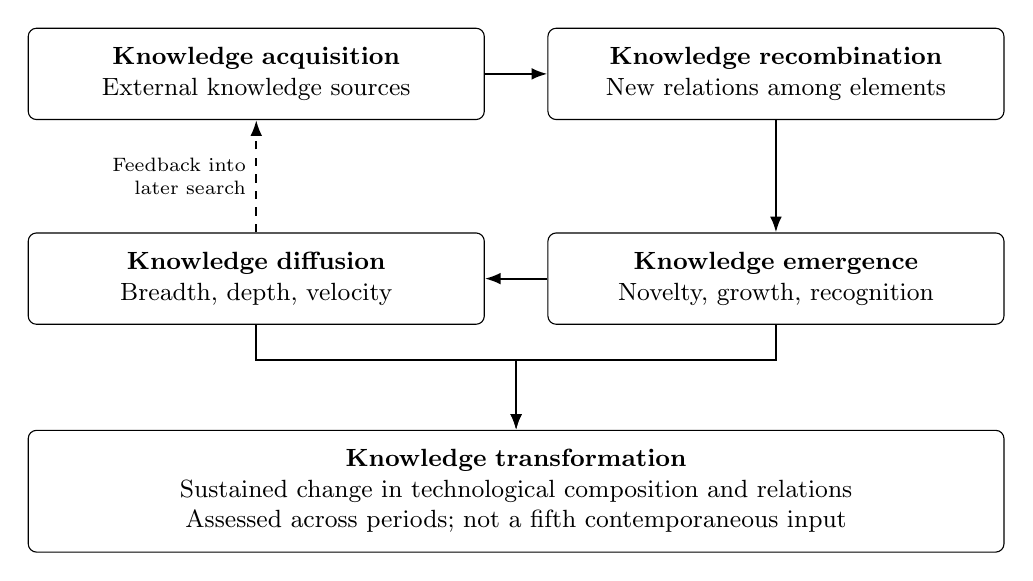
\begin{tikzpicture}[x=1cm,y=1cm]
\node[box,text width=5.3cm] (a) at (0,0) {\textbf{Knowledge acquisition}\\External knowledge sources};
\node[box,text width=5.3cm] (r) at (6.6,0) {\textbf{Knowledge recombination}\\New relations among elements};
\node[box,text width=5.3cm] (e) at (6.6,-2.6) {\textbf{Knowledge emergence}\\Novelty, growth, recognition};
\node[box,text width=5.3cm] (d) at (0,-2.6) {\textbf{Knowledge diffusion}\\Breadth, depth, velocity};
\draw[arr] (a)--(r);
\draw[arr] (r)--(e);
\draw[arr] (e)--(d);
\draw[arr,dashed] (d)--node[left,font=\scriptsize,align=right]{Feedback into\\later search}(a);
\node[box,text width=11.9cm] (t) at (3.3,-5.3) {\textbf{Knowledge transformation}\\Sustained change in technological composition and relations\\Assessed across periods; not a fifth contemporaneous input};
\draw[arr] (e.south)--++(0,-.45)-|(t.north);
\draw[arr] (d.south)--++(0,-.45)-|(t.north);
\end{tikzpicture}
\caption{Proposed knowledge evolution framework. Arrows indicate hypothesized relationships, not estimated causal effects or compulsory stages.}
\label{fig:framework}
\end{figure}


\subsection{Four process dimensions and a longitudinal outcome}
At university $u$ and period $t$, the observable process profile is
\begin{equation}
 \mathbf{x}_{ut}=(A_{ut},R_{ut},E_{ut},D_{ut})^{\mathsf T}.
 \label{eq:profile}
\end{equation}
$A$ measures documented external sourcing, $R$ unusual technical combinations,
$E$ recognized emergence, and $D$ documented diffusion. Transformation is denoted
$T_{u,t\rightarrow t+1}$ and measured separately from the change between periods.
The broader framework can be written
$\mathcal{K}_{ut}=(\mathbf{x}_{ut},T_{u,t\rightarrow t+1})$,
but the four-dimensional GMM does not include $T$ as an input. This distinction
prevents the circular procedure of using future change to construct a state and
then claiming that the state explains that same change.

The distinction also clarifies theory testing. Acquisition may increase without
recombination; recombination may occur without recognition; diffusion may be
strong even when novelty is low. Such profiles are informative counterexamples
to a simple cumulative model. The central proposition is that these dimensions
carry complementary information about changing knowledge structures. Strong
redundancy after controlling for patent volume would weaken that proposition.

\subsection{From states to trajectories}
A \emph{state} summarizes one university-period profile. A \emph{trajectory} is an
ordered sequence of profiles, states, and structural changes. We retain four
interpretive trajectory categories: \emph{Knowledge Maintenance Path},
\emph{Knowledge Expansion Path}, \emph{Knowledge Recombination Path}, and
\emph{Knowledge Transformation Path}. Maintenance denotes continuity of a core
portfolio; expansion denotes a sustained broadening of coverage; recombination
denotes recurrent unusual connections among technical elements; transformation
denotes a substantial, persistent reorganization of the portfolio.

These categories are analytic interpretations rather than four classes imposed
on the GMM. A selected model may contain fewer or more than four states, and
several states may participate in one trajectory category. A university may also
follow different paths at different times. In particular, transformation requires
direct structural evidence across at least three eligible periods; neither a
single cluster switch nor a high citation count establishes it. The terminology
does not imply a quality hierarchy: maintaining a coherent specialization can be
appropriate to an institution's research mission.

\section{Methods}\label{sec:methods}
\subsection{Patent data as technological knowledge objects}\label{sec:data}
\subsubsection{Population, coverage, and analytic unit}
The intended source is the research team's Chinese university patent database.
Its provider, extraction date, query, and field coverage must be recorded in
Table~\ref{tab:data}; they have not yet been supplied. The candidate retrieval span
in the earlier design was 2000--2025. This span remains a proposed extraction range,
not a verified observation period. The actual start, end, and mature outcome
cohorts are determined by the coverage audit and citation horizon.

The population comprises institutions in a dated, explicitly scoped Chinese
university roster and their documented historical names. Territorial and
institution-type boundaries are declared with that roster. We retain published
Chinese invention applications with a university applicant at first publication,
whether or not subsequently granted. Utility models and designs are excluded from
the primary analysis because their examination and technical disclosure differ;
utility models can be analyzed as a separate sensitivity cohort. Corporate
subsidiaries and affiliated hospitals enter only when the affiliation rule and
time-specific ownership evidence justify inclusion. Being in the university
roster does not guarantee an eligible patent portfolio.

The preferred invention unit is a simple patent family identified by a documented
family identifier and its priority set. Publication duplicates and grant versions
of the same application are collapsed first. A family is represented by its
earliest eligible public invention document, with ties resolved by a stable
publication identifier. Later continuations do not contribute text or codes to
the earlier representation. Where family identifiers are unavailable, the unit
is a deduplicated invention application, and the manuscript must say so rather
than claim family-level analysis. A family-level sensitivity analysis is then
possible only for the linked subset.

\begin{table}[tbp]\centering\fontsize{9}{11}\selectfont
\begin{tabularx}{\textwidth}{|Y|l|Y|}
\hline
\rowcolor{black} \color{white} Coverage item & \color{white} Value & \color{white} Required definition or audit\\\hline
Database/provider; extraction date & \TBD & Frozen source and query manifest\\\hline
Retrieval dates; analytic dates & \TBD & First-publication cohorts; mature end date\\\hline
Roster institutions; linked institutions & \TBD & Dated roster and name crosswalk\\\hline
Raw publication records & \TBD & Before publication/application deduplication\\\hline
Eligible invention units & \TBD & Families, or applications if families unavailable\\\hline
Eligible university-periods & \TBD & Three-year non-overlapping cohorts\\\hline
IPC subclasses; main groups & \TBD & Version-harmonized vocabulary sizes\\\hline
Usable title/abstract records & \TBD & Count and coverage percentage\\\hline
Backward-citation links & \TBD & Resolved earlier public invention units\\\hline
Forward-citation links within $H$ & \TBD & Unique family pairs, scope declared\\\hline
External citing organizations & \TBD & University-only or broader coverage\\\hline
Excluded units by reason & \TBD & Mutually exclusive first-failure counts\\\hline
\end{tabularx}
\caption{Dataset scale and coverage, to be computed from the frozen source database. No value or date range in this table is an empirical estimate.}
\label{tab:data}
\end{table}


If a unit has $m_p$ distinct university applicants, university attribution uses
$\omega_{up}=1/m_p$ for each applicant university. Thus weights sum to one over
universities for the university-attributed corpus; this is not a share of legal
ownership when firms also co-apply. A sensitivity specification divides by all
resolved applicant organizations. We report unique inventions and fractional
university totals separately. Organization names are resolved with a dated
crosswalk retaining mergers and ambiguous matches for audit.

\subsubsection{Dates, windows, and missingness}
Each unit is represented by
\begin{equation}
 p=\bigl(\mathcal{U}_p,\mathcal{C}_p,\mathbf{v}_p,
          \mathcal{B}_p,\mathcal{F}_p,\tau_p,\alpha_p,\iota_p\bigr),
\end{equation}
where $\mathcal{U}_p$ denotes applicants, $\mathcal{C}_p$ IPC codes,
$\mathbf{v}_p$ text features, $\mathcal{B}_p$ backward references,
$\mathcal{F}_p$ forward references, $\tau_p$ first publication date,
$\alpha_p$ application date, and $\iota_p$ provenance identifiers.
The main temporal clock is first publication, because it represents public
availability. Application-year results are a sensitivity analysis, not a
substitute for public-information timing. IPC codes are harmonized to a fixed
version, with ambiguous concordances reported.

We use non-overlapping three-year publication windows $W_t=[b_t,b_{t+1})$.
The preceding three years form the local historical reference window
$B_t=[b_t-3,b_t)$. A five-year forward horizon $H=5$ years measures diffusion;
early recognition uses $h_E=1$ year. These are proposed protocol settings,
not estimated data properties. A cohort contributes to the primary profile only
when every included patent has the required follow-up, so
$b_{t+1}+H\leq d_{\mathrm{extract}}$ is the conservative period eligibility rule.
The earliest cohorts without a complete historical window serve as a burn-in.

For the primary clustering cohort, require at least 20 unique inventions per
university-period, usable text for at least 80\% of its attributed mass, and
resolved citation status for at least 80\%. Thresholds of 10 and 30 inventions
and 70\% and 90\% completeness are sensitivity settings. A confirmed empty
citation list is a zero; an unavailable citation field is missing. Undefined
dimensions are not replaced by zero. Missing-dimension and small-portfolio
cohorts remain in the coverage analysis and may receive partial descriptive
profiles, but are excluded from the primary four-dimensional GMM.

\subsection{Multi-layer knowledge network construction}\label{sec:networks}
The representation is a heterogeneous multilayer system, not a multiplex graph
with identical nodes in every layer \citep{kivela2014,boccaletti2014}. IPC nodes
belong to the technological layer; patent nodes belong to the semantic and citation
layers; a patent--IPC incidence relation links their meanings. Figure~\ref{fig:pipeline}
shows how these sources enter the analysis. No weighted sum of incompatible
adjacency matrices is required.

\begin{figure}[tbp]\centering
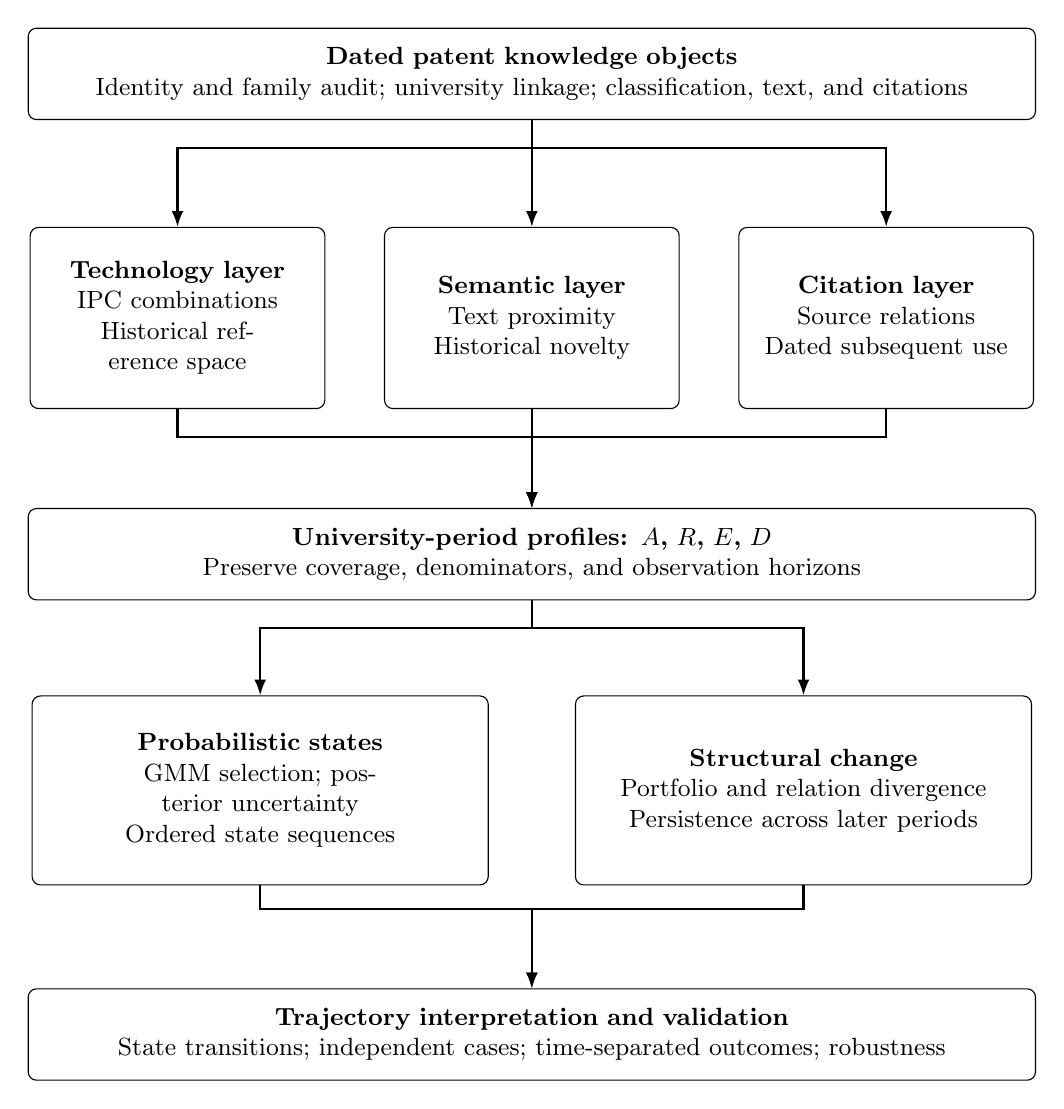
\begin{tikzpicture}[x=1cm,y=1cm]
\node[box,text width=12.3cm] (source) at (0,0) {\textbf{Dated patent knowledge objects}\\Identity and family audit; university linkage; classification, text, and citations};
\node[box,text width=3.25cm,minimum height=2.3cm] (ipc) at (-4.5,-3.1) {\textbf{Technology layer}\\IPC combinations\\Historical reference space};
\node[box,text width=3.25cm,minimum height=2.3cm] (sem) at (0,-3.1) {\textbf{Semantic layer}\\Text proximity\\Historical novelty};
\node[box,text width=3.25cm,minimum height=2.3cm] (cit) at (4.5,-3.1) {\textbf{Citation layer}\\Source relations\\Dated subsequent use};
\foreach \n in {ipc,sem,cit}{\draw[arr] (source.south)--++(0,-.35)-|(\n.north);}
\node[box,text width=12.3cm] (prof) at (0,-6.1) {\textbf{University-period profiles: $A$, $R$, $E$, $D$}\\Preserve coverage, denominators, and observation horizons};
\foreach \n in {ipc,sem,cit}{\draw[arr] (\n.south)--++(0,-.35)-|(prof.north);}
\node[box,text width=5.3cm,minimum height=2.4cm] (states) at (-3.45,-9.1) {\textbf{Probabilistic states}\\GMM selection; posterior uncertainty\\Ordered state sequences};
\node[box,text width=5.3cm,minimum height=2.4cm] (struct) at (3.45,-9.1) {\textbf{Structural change}\\Portfolio and relation divergence\\Persistence across later periods};
\draw[arr] (prof.south)--++(0,-.35)-|(states.north);
\draw[arr] (prof.south)--++(0,-.35)-|(struct.north);
\node[box,text width=12.3cm] (valid) at (0,-12.2) {\textbf{Trajectory interpretation and validation}\\State transitions; independent cases; time-separated outcomes; robustness};
\draw[arr] (states.south)--++(0,-.3)-|(valid.north);
\draw[arr] (struct.south)--++(0,-.3)-|(valid.north);
\end{tikzpicture}
\caption{Data-to-inference workflow. Transformational change is measured independently of the contemporaneous state inputs.}
\label{fig:pipeline}
\end{figure}


\subsubsection{Technology combination layer}
IPC subclasses provide the main portfolio vocabulary, while main groups provide
finer combination units. For a patent with $m_p^{C}=|\mathcal{C}_p|\geq2$ distinct
main groups, its unordered pairs receive equal total mass:
\begin{equation}
 w_{ij}^{(t)}=\sum_{p\in W_t:m_p^C\geq2}
 \frac{\ind\{i,j\in\mathcal{C}_p\}}{\binom{m_p^C}{2}},\quad i<j.
 \label{eq:cooc}
\end{equation}
University-specific networks additionally multiply each contribution by
$\omega_{up}$. Each multi-coded patent contributes one unit across pairs, reducing
inflation from records with many assigned codes. Single-code patents contribute
to node mass and portfolio composition, but not to pair weights.

For visualization, normalize with
$s_{ij}^{(t)}=w_{ij}^{(t)}/\sqrt{d_i^{(t)}d_j^{(t)}}$,
where $d_i^{(t)}=\sum_{j\ne i}w_{ij}^{(t)}$.
Edges with a zero denominator are absent. A top-10 incident-neighbor union forms
a readable map, with top-5 and top-20 alternatives; indicator calculations use
the unpruned weights. Leiden communities are descriptive technical groups
\citep{traag2019}. Map layouts are held fixed across overlays, and neither a
community label nor a two-dimensional distance is treated as a causal mechanism.

\subsubsection{Semantic layer}
The reproducible primary text representation is a character 2--4-gram TF--IDF
vector of normalized titles and abstracts. This specification accommodates Chinese
technical text without an undisclosed word-segmentation model. Training documents
come only from $B_t$; retain n-grams present in at least five reference documents
and at most 80\%, with a maximum vocabulary of 100,000 features. TF is
$1+\log n$ for positive count $n$, IDF is
$\log[(1+N)/(1+\mathrm{df})]+1$, and vectors are $L_2$ normalized.
Titles and abstracts are separated by a fixed delimiter. Claims are excluded
from the primary representation to avoid uneven availability and document-length
effects. Empty vectors are missing, not maximally novel.

Semantic similarity is
\begin{equation}
 s_{pq}=\frac{\mathbf{v}_p^{\mathsf T}\mathbf{v}_q}
 {\|\mathbf{v}_p\|_2\|\mathbf{v}_q\|_2}.
 \label{eq:semantic}
\end{equation}
A mutual 15-nearest-neighbor graph summarizes semantic structure. Retrieval for
novelty uses the full eligible historical index, not this pruned display graph.
Approximate search is permitted only with a documented recall audit against
exact search on a fixed sample. A frozen Chinese-capable sentence encoder is a
secondary representation, motivated by embedding approaches
\citep{reimers2019,sarica2020}. Its exact model, tokenizer, revision, training-data
limitations, and inference parameters must be recorded before it is used.
Modern pretrained representations are treated as retrospective sensitivities
unless their historical information boundary can be established.

\subsubsection{Citation diffusion layer}
Citation edges point from a cited predecessor to a citing descendant, the direction
of documented knowledge reuse. Collapse duplicate family-pair citations, remove
within-family links, and retain only relations whose predecessor was already
public. Same-day or inconsistent-date references are retained in an audit file
and excluded from the time-directed graph. Self-citations are identified by
overlap of canonical applicant-organization sets; the primary diffusion measure
excludes those edges.

A database containing only university patents supports university-to-university
diffusion. A broader claim requires forward citations from all covered
organizations, together with their publication dates, identifiers, and IPC fields.
Two-step diffusion additionally requires the descendants' outgoing reuse links.
Where these are not available, depth is unavailable and the full $D$ score cannot
be reported. A two-component breadth--velocity score may be reported as a
separately named sensitivity measure, never silently substituted for $D$.

\subsection{Knowledge evolution profile extraction}\label{sec:indicators}
Let $P_{ut}$ be the focal university-period portfolio and
$M_{ut}=\sum_{p\in P_{ut}}\omega_{up}$. The following definitions retain natural
zeros while distinguishing absent evidence. All normalized components lie in
$[0,1]$; their direction is intensity of an observable process, not research quality.
For a dimension $j$, $P_{ut}^{j}$ contains only inventions with verified required
fields, and $M_{ut}^{j}=\sum_{p\in P_{ut}^{j}}\omega_{up}$ is its valid attributed
mass. Report $M_{ut}^{j}/M_{ut}$ for every dimension; missing records never enter
an indicator denominator as observed zeros.

\subsubsection{Knowledge acquisition: external sourcing and source diversity}
For each patent, identify resolved backward-cited inventions whose applicant sets
do not overlap its own. Let $q_{ut}$ be the weighted proportion of focal inventions
with at least one such external reference. Fractionally allocate each external
reference over its IPC subclasses and normalize the aggregate to a source
distribution $\pi_{ut,k}$. Let $K_t$ cover the fixed, version-harmonized source
subclass vocabulary, including a recorded unresolved-code category; this same
vocabulary contains all subclasses receiving source mass. Define
\begin{align}
 q_{ut}&=\frac{\sum_{p\in P_{ut}^{A}}\omega_{up}
           \ind\{|\mathcal{B}^{\mathrm{ext}}_p|>0\}}{M_{ut}^{A}},\\
 A_{ut}&=q_{ut}\left[\frac12+\frac12
       \frac{-\sum_{k=1}^{K_t}\pi_{ut,k}\log\pi_{ut,k}}{\log K_t}\right].
 \label{eq:acquisition}
\end{align}
The entropy term is zero when $K_t\leq1$. With confirmed absence of external
references, $q=A=0$ and source entropy is recorded as undefined rather than
interpreted as a concentrated distribution. The positive baseline inside the
bracket distinguishes narrow external sourcing from no sourcing at all.
The two components are always reported alongside the composite. This is a
documented-sourcing proxy, not a direct measurement of absorptive capacity
\citep{cohen1990,shannon1948,stirling2007}.

\subsubsection{Knowledge recombination: historical pair rarity}
For an unordered IPC-main-group pair $(i,j)$, let $c_{ij,t}^{-}$ be its fractional
co-occurrence mass in $B_t$. Let $L_t$ be the fixed vocabulary size established
before the focal window, augmented by one out-of-vocabulary category, and
$Q_t=\binom{L_t}{2}$. Define the smoothed pair probability and its normalized surprise:
\begin{align}
 p_{ij,t}^{-}&=\frac{c_{ij,t}^{-}+\alpha}
 {\sum_{a<b}c_{ab,t}^{-}+\alpha Q_t},\quad \alpha=\tfrac12,\\
 r_{ij,t}&=\clip_{[0,1]}\left[
 \frac{-\log p_{ij,t}^{-}}{
 -\log\{\alpha/(\sum_{a<b}c_{ab,t}^{-}+\alpha Q_t)\}}\right],\\
 R_{ut}&=\frac{\sum_{p\in P_{ut}^{(2)}}\omega_{up}
       |\mathcal{L}_p|^{-1}\sum_{(i,j)\in\mathcal{L}_p}r_{ij,t}}
       {\sum_{p\in P_{ut}^{(2)}}\omega_{up}}.
 \label{eq:recombination}
\end{align}
$\mathcal{L}_p$ is the set of distinct, valid mapped pairs and $P_{ut}^{(2)}$
contains patents with at least one such pair. A window with no historical pair
mass is ineligible. Newly introduced classifications are mapped through the
fixed concordance; unresolved new codes use the single out-of-vocabulary category,
whose prevalence is reported and excluded in sensitivity analysis. Self-pairs
created by that mapping are removed. A university with no eligible pair is
assigned missing $R$, and its multi-code share is reported separately.

Rarity is not a guarantee of novelty or usefulness
\citep{fleming2001,youn2015,verhoeven2016}. We therefore inspect the distribution
of pair support, compare first-seen-pair rates, and audit text examples. A
patent-count-preserving permutation of IPC incidence supplies a reference
distribution for combinations that can arise from marginal class frequencies.

\subsubsection{Knowledge emergence: novelty, growth, and recognition}
For patent $p$, semantic novelty relative to the historical reference corpus is
\begin{equation}
 n_{p,t}=1-\max_{q\in B_t}s_{pq},\qquad 0\leq n_{p,t}\leq1.
 \label{eq:novelty}
\end{equation}
Near-duplicate members of the same family cannot be historical comparators.
Let $\rho_{k,t}$ denote the fractional share of subclass $k$ in the entire
observed reference population during $W_t$, and $\rho_{k,t}^{-}$ its share in
$B_t$. The term ``reference population'' means the university corpus unless
broader patent coverage is documented. Relative growth is
\begin{equation}
 g_{k,t}=\max\left\{0,
 \frac{\rho_{k,t}-\rho_{k,t}^{-}}{\rho_{k,t}+\rho_{k,t}^{-}+\varepsilon}\right\},
 \quad\varepsilon=10^{-12},\qquad
 g_{p,t}=|\mathcal{C}^{S}_p|^{-1}\sum_{k\in\mathcal{C}^{S}_p}g_{k,t},
 \label{eq:growth}
\end{equation}
where $\mathcal{C}^{S}_p$ contains subclasses. Growth based on shares limits the
effect of corpus-wide expansion; raw counts and minimum support are still audited.
An unseen field can reach high proportional growth with few documents, so results
are repeated after requiring at least 10 current-window inventions per field.

Let $z_p=\ind\{p\text{ receives an external citation within }h_E\}$.
The primary recognized-emergence score is the mean of patent-level products:
\begin{equation}
 E_{ut}=\frac{\sum_{p\in P_{ut}^{E}}\omega_{up}
              n_{p,t}g_{p,t}z_p}
              {M_{ut}^{E}}.
 \label{eq:emergence}
\end{equation}
This retains the earlier \emph{novelty $\times$ growth $\times$ recognition}
idea while preventing three unrelated patent subsets from generating a high
score through a product of aggregate means. The component means, their dependence,
and the fraction with a nonzero product are reported. A zero can reflect lack
of any one component. The precursor
$E^{\mathrm{pre}}_{ut}=\sum\omega_{up}n_{p,t}g_{p,t}/\sum\omega_{up}$
omits later recognition and is evaluated separately for early-use questions.
Coherence checks inspect whether high-scoring records share interpretable technical
content; the score alone does not establish an emerging technology in the full
sense of \citet{rotolo2015}.

\subsubsection{Knowledge diffusion: breadth, depth, and velocity}
Let $\mathcal{F}_p^H$ be direct external citing units first published within
$(\tau_p,\tau_p+H]$. Define organizational breadth $b_p$ as the number of distinct
external applicant organizations in this set. Also report citing-field entropy
and the external-university share as descriptive breadth components. Let
$\mathcal{F}_p^{(2),H}$ contain unique second-step descendants that lie on a
time-respecting path within the same horizon; direct descendants and the focal
family are excluded. Define depth and velocity by
\begin{equation}
 \ell_p=|\mathcal{F}_p^{(2),H}|,\qquad
 v_p=\begin{cases}
 1-\Delta_p/H,&\mathcal{F}_p^H\ne\varnothing,\\
 0,&\mathcal{F}_p^H=\varnothing,
 \end{cases}
 \label{eq:diffusion-components}
\end{equation}
where $\Delta_p$ is the time in years to first external citation. Citation arrival
at the horizon has zero velocity; zero-citation records remain in the denominator.
Depth reflects bounded network reach, not an identified causal chain of learning.
Time-to-first-citation and later accumulation warrant separate interpretation
\citep{huang2019}.

For $z\in\{b,\ell,v\}$, use a zero-preserving field--cohort transform:
\begin{equation}
 \phi_{f,t}^{z}(x)=\begin{cases}
 0,&x=0,\\
 \{\#(0<z_q<x)+\tfrac12\#(z_q=x)\}/N_{f,t}^{z,+},&x>0.
 \end{cases}
 \label{eq:ranknorm}
\end{equation}
The comparison set contains positive observations in the same primary IPC
subclass and three-year cohort. If fewer than 30 positive observations are
available, back off to the IPC section and then to the whole cohort; the chosen
level is recorded. Field assignment uses the designated primary code, or a
deterministic documented code order if that field is absent. If the final
comparison set has no positives, all verified observations have value zero.
Then
\begin{equation}
 D_{ut}=\frac{1}{3M_{ut}^{D}}
 \sum_{p\in P_{ut}^{D}}\omega_{up}
 \left[\phi^{b}_{f,t}(b_p)+\phi^{\ell}_{f,t}(\ell_p)+\phi^{v}_{f,t}(v_p)\right].
 \label{eq:diffusion}
\end{equation}
Equal component weights are transparent design choices. Raw components and
alternative weights are retained because percentile normalization can conceal
large absolute changes.

\subsection{Dynamic pattern identification}\label{sec:patterns}
\subsubsection{Gaussian mixture states}
The primary GMM is fitted to all eligible university-period profiles after
global dimension-wise standardization. Each row has equal weight, so the fitted
population is university-periods; we additionally fit weights summing to one
per university to assess effects of unequal panel length. Highly active
institutions do not receive weight proportional to their patent volume.
The model is
\begin{equation}
 f(\mathbf{z}_{ut})=\sum_{k=1}^{K}\pi_k
 \mathcal{N}(\mathbf{z}_{ut}\mid\boldsymbol\mu_k,\boldsymbol\Sigma_k),
 \qquad \sum_k\pi_k=1.
 \label{eq:gmm}
\end{equation}
Evaluate $K=1,\ldots,8$ using full and diagonal covariance matrices, covariance
regularization $10^{-6}$, and 50 seeded initializations. Minimize
$\mathrm{BIC}=-2\log\widehat L+d\log n$ \citep{schwarz1978}.
For four variables, $d=15K-1$ for full covariance and $d=9K-1$ for diagonal
covariance. Models with a component below 3\% of rows are flagged; no such
component is accepted without an explicit stability and substantive assessment.
BIC is a selection aid under an approximate distributional model, not proof of
natural university types \citep{fraley2002,scrucca2016}.

Assign posterior responsibilities $\gamma_{utk}$ and descriptive labels
$\widehat s_{ut}=\arg\max_k\gamma_{utk}$. Report maximum posterior probability
and normalized posterior entropy. A maximum below 0.60 marks an uncertain
assignment; this is a reporting threshold, not a deletion rule. Bootstrap the
entire university trajectory, refit standardization and the GMM, and align
components to the reference solution using minimum-distance centroid matching.
If $K$ changes, report that change and compare co-assignment rather than forcing
one-to-one labels. Assess adjusted Rand index, clusterwise overlap, and
silhouette descriptions \citep{hubert1985,hennig2007,rousseeuw1987}. Zeros,
boundedness, and skewness may violate Gaussian assumptions, so transformed GMMs
and $k$-means are explicit sensitivity analyses.

\subsubsection{State transitions and uncertainty}
For consecutive eligible periods with no intervening missing window, define
\begin{equation}
 n_{ij}=\sum_{u,t}\ind\{\widehat s_{ut}=i,\widehat s_{u,t+1}=j\},
 \quad n_{i+}=\sum_jn_{ij},\quad
 \widehat P_{ij}=\frac{n_{ij}}{n_{i+}}.
 \label{eq:markov}
\end{equation}
Rows with no transitions are undefined. Table~\ref{tab:markov} reports counts,
probabilities, and university-bootstrap intervals. The sensitivity statistic
$\widetilde n_{ij}=\sum_{u,t}\gamma_{uti}\gamma_{u,t+1,j}$ describes posterior-weighted
co-occurrence under a factorization assumption; it is not an inferred joint
transition posterior. Separate estimates for early and late windows assess
nonstationarity. Comparison with a second-order model evaluates whether the
previous state improves held-out log loss, using a fixed label space.
Stationary distributions are not interpreted unless time-homogeneity is credible.

Whole-university resampling preserves dependence among adjacent transitions
\citep{efron1979}. We use 1,000 replicates for final intervals and record failed
fits. When null transition opportunities are evaluated, shuffle period order
within university while retaining each university's state frequencies, and
compare persistence and selected pathway counts to that null. Small cells are
reported as uncertain, not converted into general developmental laws.

\subsubsection{Transformation as sustained structural change}
Let $\mathbf{a}_{ut}$ be the fractional IPC-subclass portfolio distribution, and
$\mathbf{r}_{ut}$ the normalized distribution of IPC-pair mass, both represented
on a shared vocabulary. Define
\begin{align}
 \JSD(\mathbf{p},\mathbf{q})&=\tfrac12\KL(\mathbf{p}\|\mathbf{m})+
                   \tfrac12\KL(\mathbf{q}\|\mathbf{m}),\quad
                   \mathbf{m}=\tfrac12(\mathbf{p}+\mathbf{q}),\\
 T_{u,t\rightarrow t+1}&=\frac{\JSD(\mathbf{a}_{ut},\mathbf{a}_{u,t+1})+
                    \JSD(\mathbf{r}_{ut},\mathbf{r}_{u,t+1})}{2\log2}.
 \label{eq:transformation}
\end{align}
Natural logarithms yield $T\in[0,1]$ \citep{lin1991}. An unavailable pair
distribution makes the two-layer $T$ missing; a composition-only divergence is
reported separately. Diversity and field distance can provide complementary
interpretation, but are not equivalent to transformation
\citep{stirling2007,porter2009}.

A change exceeds finite-portfolio noise when it lies above the 95th percentile
of a within-university null obtained by pooling the adjacent periods' patents
and permuting their period labels while preserving period sample sizes.
Repeat with portfolio-size-matched subsamples to assess output growth effects.
Call it \emph{sustained} only when, in the next eligible period, the new profile
is closer to period $t+1$ than to period $t$, using the same two-layer divergence,
and remains distinguishable from the old profile under the permutation test.
At least three consecutive periods are therefore required. A high $T$ caused
mainly by name resolution, classification revision, or a merger is treated as
an organizational or measurement event. Claims of a technological paradigm
shift require additional substantive evidence beyond this statistic
\citep{dosi1982,funk2017}.

\subsection{Empirical validation and robustness}\label{sec:validation}
Validation addresses construct distinctness, stability, and independent information.
First, report pairwise Spearman correlations, zero shares, and coverage dependence
for all dimensions and components. Compare each dimension with log patent
volume, portfolio entropy, field composition, and period. Second, conduct blinded
case assessment of the original patent descriptions, references, and chronology.
Third, evaluate whether profiles add information for outcomes that do not reuse
the same observation interval.

For temporal evaluation, set a portfolio-level availability time
$a_t=b_{t+1}+H$. All profile inputs must be available by $a_t$. Outcomes count
new external citing organizations during $(a_t,a_t+3]$ that were not observed
as users of the focal portfolio by $a_t$, and separately assess portfolio change
in publication windows beginning after $a_t$. Training outcomes must finish
before the test portfolio's availability time. Refit text vocabulary, scaling,
normalization references, and any GMM within each training split; no future
population percentile or final-period model is transferred backward in time.
If enough separated mature windows are unavailable, temporal validation is
declared infeasible rather than replaced by a random row split.

A baseline includes patent volume, average age, university effects where
identifiable, period, and field composition. An extended count model adds
$A,R,E,D$, using Poisson pseudo-maximum likelihood and university-clustered
uncertainty. Report held-out deviance and mean absolute error; for a binary
sustained-change outcome report log loss, calibration, and precision--recall
performance. To address early monitoring, a separate model uses only information
available at the end of $W_t$, including $E^{\mathrm{pre}}$ and age-observed
diffusion, and is not presented as the same matured four-dimensional profile.
Prediction improvements are associations, not evidence that changing an
indicator will cause an outcome.

For case assessment, select central and uncertain trajectories across model
states and portfolio-size strata, before reading validation outcomes. Aim for
24 cases and at least two independent technically qualified raters, subject to
the number of eligible trajectories. Show dated evidence without model labels,
institution ranking, or score summaries. Raters assess source continuity,
technical combination, emerging direction, and sustained structural change.
Report raw agreement and Cohen's kappa with intervals for prespecified nominal
labels \citep{cohen1960}; preserve initial ratings and document adjudication.
Cases can disconfirm a model interpretation, not merely illustrate it.

Table~\ref{tab:robustness} defines sensitivity families: record unit, attribution,
representation, thresholds, clustering, time windows, citation coverage, and
indicator components. Report effect changes, assignment agreement, and coverage
changes rather than a single ``robust'' label. Prespecified secondary
associations use Benjamini--Hochberg false-discovery-rate adjustment
\citep{benjamini1995}. Cluster discovery remains exploratory. Appendix A
specifies implementation details and the audit record needed to reproduce each
table from the source data.

\section{Results}\label{sec:results}
\textit{Empirical reporting status.} This section contains the complete reporting
structure and interpretive logic for the planned analysis. Numerical entries and
data-dependent statements cannot be completed until the database is processed.
The marked fields below must be replaced by verified outputs; the existence,
direction, and strength of a result remain open.

\subsection{Coverage and technological knowledge landscape}
The final analytic population comprises \pending{number of universities},
\pending{number of unique inventions}, and \pending{number of university-periods}
over \pending{verified mature publication cohorts}. Table~\ref{tab:data} separates
raw retrieval from invention-level deduplication and profile eligibility. The
principal reasons for exclusion are \pending{ranked exclusion reasons and counts}.
Citation and text coverage vary by \pending{observed field, period, and institution
patterns}. This accounting establishes the population to which subsequent
descriptions apply. In particular, a predominance of highly active institutions
after eligibility filtering would narrow the scope from Chinese universities
generally to universities with sufficiently observed patent activity.

Figure~\ref{fig:map} is reserved for the common technological map and time overlays.
Its node count, edge count, community count, and retained mass are
\pending{network statistics}. The overlay comparison reports entry, persistence,
and exit of technical subclasses, while keeping node coordinates fixed. An increase
in the number of visible areas is interpreted alongside portfolio size and rarefied
class coverage. It cannot by itself establish diversification, because a larger
sample has more opportunities to include infrequent classes. Semantic neighbors
provide a second view of the technical content; discrepancies between the two
representations identify records requiring substantive inspection.

\begin{figure}[tbp]\centering
\figpanel{0.48\textwidth}{A. Common technological space}{
Data required: IPC nodes and weighted pairs.\\[.6em]
Position: one fixed reference layout.\\
Node area: fractional invention mass.\\
Edges: normalized co-occurrence.\\[.6em]
\textbf{Empirical map not yet computed.}}
\hfill
\figpanel{0.48\textwidth}{B. Period overlays}{
Data required: period-specific IPC mass.\\[.6em]
Reuse panel A coordinates.\\
Show entry, persistence, and exit.\\
Report retained mass and omitted nodes.\\[.6em]
\textbf{Empirical overlays not yet computed.}}
\caption{Technological knowledge space: analysis specification awaiting source data. The panels contain no synthetic nodes, invented clusters, or empirical coordinates.}
\label{fig:map}
\end{figure}


\subsection{Distribution and distinctness of evolution dimensions}
Table~\ref{tab:descriptive} reports the full distribution of the four dimensions,
including medians, interquartile ranges, zeros, and valid denominators. The observed
rank order of average intensities is \pending{rank order}, but comparisons across
dimensions are secondary because each score has a different substantive meaning.
More informative are within-dimension variation and the joint profiles. The
correlation between recombination and recognized emergence is
\pending{Spearman correlation and interval}; the correlation between emergence
and diffusion is \pending{Spearman correlation and interval}. These associations
must be interpreted with the shared recognition component in mind.

After accounting for portfolio size, period, and field composition, the remaining
association between the four scores and output volume is
\pending{adjusted associations}. Weak residual distinctions would indicate that
the profile largely repackages established size and field effects. Conversely,
substantial variation among size- and field-comparable portfolios would support
the usefulness of the relational measurements. Neither interpretation is selected
in advance. Component-level results also distinguish low emergence due to limited
novelty from low emergence due to delayed recognition; equal composite values can
otherwise conceal different processes.

\begin{table}[tbp]\centering\fontsize{9}{11}\selectfont
\begin{tabularx}{\textwidth}{|Y|c|c|c|c|c|c|}
\hline
\rowcolor{black} \color{white} Dimension & \color{white} Valid $n$ & \color{white} Mean & \color{white} SD & \color{white} Median & \color{white} IQR & \color{white} Zero \%\\\hline
Acquisition ($A$) & \TBD & \TBD & \TBD & \TBD & \TBD & \TBD\\\hline
Recombination ($R$) & \TBD & \TBD & \TBD & \TBD & \TBD & \TBD\\\hline
Emergence ($E$) & \TBD & \TBD & \TBD & \TBD & \TBD & \TBD\\\hline
Diffusion ($D$) & \TBD & \TBD & \TBD & \TBD & \TBD & \TBD\\\hline
\end{tabularx}
\caption{Distribution of the four process dimensions across eligible university-periods. Each row also requires observed minimum, maximum, missing count, and component summaries in the accompanying output file.}
\label{tab:descriptive}
\end{table}


\subsection{Probabilistic states and interpreted trajectories}
Among the candidate models, the selected specification has
\pending{selected $K$ and covariance structure}, with
\pending{BIC difference from the nearest admissible alternative}. Table~\ref{tab:gmm}
reports component prevalence and the original-scale profile means. The proportion
of assignments below the posterior-confidence threshold is
\pending{uncertain assignment percentage}. Bootstrap agreement is
\pending{ARI and interval}, and the frequency with which the selected state count
recurs is \pending{selection frequency}. These quantities determine how strongly
the state solution can be interpreted.

Figure~\ref{fig:states} combines the observed state profiles with an ordered
trajectory view. A maintenance interpretation requires stable technical
composition; an expansion interpretation requires persistent coverage gains;
a recombination interpretation requires repeated unusual pair formation supported
by text; a transformation interpretation additionally requires the structural and
persistence tests. The resulting number of supported trajectory categories is
\pending{supported categories and counts}. Where profiles overlap, uncertain or
mixed trajectories remain visible. A state is not renamed ``transformation'' merely
because it has the largest values on all four dimensions.

\begin{table}[tbp]\centering\fontsize{9}{11}\selectfont
\begin{tabularx}{\textwidth}{|Y|c|c|c|c|c|c|}
\hline
\rowcolor{black} \color{white} Selected component & \color{white} Share & \color{white} $\bar A$ & \color{white} $\bar R$ & \color{white} $\bar E$ & \color{white} $\bar D$ & \color{white} Max. post.\\\hline
$S_1$ & \TBD & \TBD & \TBD & \TBD & \TBD & \TBD\\\hline
$\vdots$ & $\vdots$ & $\vdots$ & $\vdots$ & $\vdots$ & $\vdots$ & $\vdots$\\\hline
$S_{\widehat K}$ & \TBD & \TBD & \TBD & \TBD & \TBD & \TBD\\\hline
\end{tabularx}
\caption{GMM state characteristics, with the number of rows determined by model selection. Means require university-bootstrap intervals; ``Max. post.'' is the mean maximum posterior assignment probability.}
\label{tab:gmm}
\end{table}


\begin{figure}[tbp]\centering
\figpanel{0.48\textwidth}{A. Evolution profile space}{
Data required: $A,R,E,D$ and posteriors.\\[.6em]
Show original-scale state profiles.\\
Add university-bootstrap intervals.\\
Use PCA only for a secondary view.\\[.6em]
\textbf{No state centroids estimated.}}
\hfill
\figpanel{0.48\textwidth}{B. University trajectories}{
Data required: consecutive period states.\\[.6em]
Horizontal axis: publication window.\\
Rows: prespecified sampled universities.\\
Mark uncertain and missing periods.\\[.6em]
\textbf{No trajectories assigned.}}
\caption{Evolution profile and trajectory displays: analysis specification. State labels must follow the fitted model, and the trajectory interpretation must use independent structural evidence.}
\label{fig:states}
\end{figure}


\subsection{Transitions and sustained structural transformation}
Table~\ref{tab:markov} reports transitions among the fitted states. The overall
same-state persistence rate is \pending{rate and interval}, compared with
\pending{within-university permutation expectation}. The best-supported off-diagonal
transitions are \pending{transitions, counts, probabilities, and intervals}.
These estimates apply to universities observed in consecutive eligible periods;
they do not include jumps over missing windows. Early- and late-period matrices
differ by \pending{estimated divergence or stability diagnostic}, determining
whether an aggregate matrix is an adequate summary.

The earlier draft suggested that recombination could serve as an intermediate
route toward transformation. The appropriate test counts ordered sequences with
recombination evidence followed by independently established sustained structural
change, and compares them with frequency-preserving shuffled sequences. The
observed contrast is \pending{effect size and interval}. A nonpositive or unstable
contrast would leave that proposed mechanism unsupported. Even a positive contrast
would establish temporal association rather than causation. Figure~\ref{fig:transitions}
places transition frequencies beside structural change and persistence so that
state switching cannot be mistaken for transformation.

\begin{table}[tbp]\centering\fontsize{9}{11}\selectfont
\begin{tabularx}{\textwidth}{|Y|c|c|c|c|}
\hline
\rowcolor{black} \color{white} From / to & \color{white} $S_1$ & \color{white} $\cdots$ & \color{white} $S_{\widehat K}$ & \color{white} Row count\\\hline
$S_1$ & \TBD & $\cdots$ & \TBD & \TBD\\\hline
$\vdots$ & $\vdots$ & $\ddots$ & $\vdots$ & $\vdots$\\\hline
$S_{\widehat K}$ & \TBD & $\cdots$ & \TBD & \TBD\\\hline
\end{tabularx}
\caption{First-order transition matrix among fitted knowledge-profile states. Each populated probability cell must include its count and 95\% university-bootstrap interval; only defined rows sum to one.}
\label{tab:markov}
\end{table}


\begin{figure}[tbp]\centering
\figpanel{0.48\textwidth}{A. Observed state movement}{
Data required: transition count matrix.\\[.6em]
Rows: origin state. Columns: next state.\\
Display probabilities and row counts.\\
Keep low-support cells visible.\\[.6em]
\textbf{No transition rates estimated.}}
\hfill
\figpanel{0.48\textwidth}{B. Structural transformation}{
Data required: divergence and null draws.\\[.6em]
Plot $T$ against its size-matched null.\\
Mark persistence in the third period.\\
Separate merger and coding events.\\[.6em]
\textbf{No transformation events confirmed.}}
\caption{Transition and transformation evidence: analysis specification. The second panel supplies the structural test required for a transformation interpretation of the first.}
\label{fig:transitions}
\end{figure}


\subsection{Independent validation, cases, and robustness}
In the temporal evaluation, the extended profile model changes held-out deviance
by \pending{change and uncertainty} relative to the volume--field baseline, with
\pending{calibration and absolute-error results}. The mature retrospective model
and the early-information model are reported separately. A gain present only when
later citation information is available would support retrospective description
but would not justify an early-warning claim.

Independent raters assess \pending{number of cases}; agreement is
\pending{raw agreement, kappa, and intervals}. The most informative disagreements
concern \pending{evidence-grounded disagreement themes}. Each selected case traces
named technical problems, representative invention identifiers, predecessor
relations, and later use. A successful explanation must identify what changed
in the technology, not simply restate a high score. Cases in which the automated
label is rejected are retained to identify construct boundaries.

Table~\ref{tab:robustness} and Figure~\ref{fig:validation} summarize the effects of
alternative assumptions. The largest changes in state membership or transition
estimates arise under \pending{settings and magnitudes}. Stability is assessed on
the common eligible sample, while sample changes are reported separately. Any
major dependence on a single representation, sparse citation coverage, or the
portfolio-size threshold limits the generality of the trajectory interpretation.
The final conclusion must therefore be calibrated to the least secure link among
coverage, construct validity, assignment stability, and independent evidence.

\begin{table}[tbp]\centering\fontsize{9}{11}\selectfont
\begin{tabularx}{\textwidth}{|P{3.1cm}|Y|P{2.4cm}|}
\hline
\rowcolor{black} \color{white} Test family & \color{white} Alternative and comparison & \color{white} Observed result\\\hline
Invention unit & Application versus family; overlap and profile change & \TBD\\\hline
Attribution & University-fractional versus all-applicant and full counts & \TBD\\\hline
Representation & IPC resolution; TF--IDF versus frozen encoder & \TBD\\\hline
Clustering & GMM covariance, transformed GMM, $k$-means; selected $K$ and ARI & \TBD\\\hline
Window length & Non-overlapping 2-, 3-, and 4-year cohorts; sequence agreement & \TBD\\\hline
Outcome horizon & 3 versus 5 years on common mature cohorts & \TBD\\\hline
Eligibility & Minimum 10/20/30 inventions; completeness 70/80/90\% & \TBD\\\hline
Citation scope & Self-citations; examiner status; external coverage & \TBD\\\hline
Components & $E^{\mathrm{pre}}$; separate $D$ components; weight sensitivity & \TBD\\\hline
Independent evidence & Future use; blinded cases; structural persistence & \TBD\\\hline
\end{tabularx}
\caption{Robustness and validation results, pending computation. Each row requires the common-sample size, effect or agreement estimate, interval where applicable, and change in coverage.}
\label{tab:robustness}
\end{table}


\begin{figure}[tbp]\centering
\figpanel{0.48\textwidth}{A. Incremental information}{
Data required: temporally held-out outputs.\\[.6em]
Compare volume--field baseline with profile.\\
Report prediction error and calibration.\\
Separate mature and early-information models.\\[.6em]
\textbf{No validation gain observed yet.}}
\hfill
\figpanel{0.48\textwidth}{B. Sensitivity and case agreement}{
Data required: refits and blinded ratings.\\[.6em]
Display effect changes with intervals.\\
Show state agreement and sample retention.\\
Include cases that reject model labels.\\[.6em]
\textbf{No robustness claim established.}}
\caption{Validation summary: analysis specification. All comparisons require recorded outcome windows, denominators, and uncertainty; the panels contain no illustrative performance values.}
\label{fig:validation}
\end{figure}


\FloatBarrier
\section{Discussion}\label{sec:discussion}
\subsection{Knowledge evolution as a relational and temporal construct}
The principal theoretical value of the framework is the separation of processes
that are often compressed into an undifferentiated account of innovation.
Acquisition concerns the relation to prior knowledge, recombination concerns
relations among technical elements, emergence concerns the alignment of novelty,
growth, and recognition, and diffusion concerns later patterns of documented use.
Transformation concerns whether these activities are accompanied by sustained
changes in the organization of a technological portfolio. Their separation creates
testable possibilities for divergence as well as accumulation.

This formulation refines a sequential interpretation of knowledge evolution.
An external knowledge source may support routine specialization; an unusual
combination may fail to attract recognition; and established technical knowledge
may diffuse widely without being novel. The empirical question is whether
particular configurations and sequences recur more often than their marginal
frequencies predict. If they do, the framework provides an evidence structure
for explaining those trajectories. If they do not, its value remains descriptive,
and stronger mechanism claims should be withheld. Process vocabulary is useful
only when the observable relations remain connected to its theoretical meaning.

Transformation is particularly vulnerable to overstatement. In the present
design, portfolio divergence is a measurable form of structural reorganization,
not an automatic indicator of a technological revolution. A move into an
established field can transform one university's portfolio without changing the
global frontier. Conversely, a scientifically important invention may leave the
institution's aggregate composition largely unchanged. This distinction locates
the contribution at the organization--knowledge-system interface and preserves
the broader meaning of technological trajectories in evolutionary innovation
theory \citep{dosi1982}.

\subsection{Contribution to information science and knowledge organization}
The disciplinary contribution lies in connecting knowledge representation with
temporally accountable interpretation. The same invention is linked to a formal
classification, a text neighborhood, a set of predecessors, and a later citation
neighborhood. Rather than merging these into an opaque similarity score, the
framework records which relation supports which inference. A surprising IPC pair
supports a combination claim; a remote semantic neighbor supports a content
novelty claim; a later citing organization supports a bounded diffusion claim.
Disagreement across these views is preserved as a source of analytical evidence.

This approach builds on patent mapping, rather than claiming its invention
\citep{kay2014,leydesdorff2014,yan2017}. Its proposed extension is to connect maps,
profiles, and trajectories through an explicit unit of observation and a declared
time boundary. That connection matters for information analysis because maps are
frequently used to support claims about change that their visual construction
does not itself establish. Keeping graphical layouts separate from structural
statistics makes those claims inspectable and reproducible.

The framework also treats knowledge organization as historically situated.
Classifications change, technical language shifts, and a relation that is unusual
at one time may become routine later. Historical reference windows and fixed
version mappings provide a controlled basis for studying that evolution, while
the audit retains uncertainty introduced by retrospective metadata. The result
is a research design for organizing evidence about change, with a clear route
from an aggregate description back to the patent records supporting it.

\subsection{Implications for university innovation governance}
The framework suggests a diagnostic use of patent information. A university with
strong source breadth but limited recombination poses a different management
question from one that repeatedly produces unusual combinations with little
subsequent recognition. A stable specialist portfolio raises yet another question:
whether continuity reflects productive accumulation or an inability to respond
to changing technical opportunities. Such interpretations require substantive
context; no score determines the answer by itself.

The four trajectory categories can organize that inquiry without ranking
institutions along a single developmental ladder. Maintenance may justify
continued support for long-term technical capabilities. Expansion may call for
attention to coherence and resource dispersion. Recombination may motivate
investigation of the facilities and expertise needed to test unusual technical
connections. Transformation may require sustained support and a review of
organizational discontinuities. These are conditional questions for governance,
not interventions shown to work by the proposed observational analysis.

Any policy-facing use should display coverage, uncertainty, and representative
evidence alongside aggregate profiles. A weakly observed university should not
be labelled as lacking diffusion merely because external citations are absent
from the database. Similarly, a broad profile should not automatically be rated
above a specialized one. This restraint is consistent with responsible use of
research metrics, where quantitative evidence supports contextual judgment
\citep{hicks2015}.

\subsection{Limitations and boundary conditions}
Several boundaries remain even after the empirical implementation is completed.
First, patents cover a selective part of university knowledge production. The
framework cannot represent all scientific contributions, tacit expertise, open
software, or inventions protected through other means. It does not measure
commercialization, licensing success, or market value without additional evidence.
Second, citations record formal prior-art relationships, including examiner
contributions; they do not directly observe learning or contractual transfer
\citep{alcacer2006}. These limitations restrict both acquisition and diffusion
interpretations.

Third, available data may be narrower than the conceptual network. In particular,
university-only forward citations describe a bounded academic technological
subsystem, and missing descendant links can prevent depth measurement. Fourth,
novelty is relative to the observed historical corpus and chosen representation.
It cannot establish worldwide novelty, nor replace legal examination or technical
expertise. Character-based similarity can be sensitive to terminology; pretrained
encoders introduce different training and temporal uncertainties.

Fifth, the multiplicative emergence score deliberately penalizes absence of any
component and will often be zero. That property makes it interpretable as
recognized joint evidence, but unsuitable as the sole measure of early emerging
directions. Sixth, the GMM approximates a continuous and possibly non-Gaussian
space; unstable or overlapping components may not support categorical summaries.
Seventh, a first-order transition matrix can miss longer memory, changing
institutional conditions, and cohort effects. Finally, retrospective profiles
and subsequent structural changes remain observational. Institutional strategy,
staff recruitment, collaboration, and policy changes can affect both. The analysis
can identify patterned associations and cases for explanation, but cannot isolate
causal mechanisms without additional designs.

\section{Conclusion}\label{sec:conclusion}
Understanding technological knowledge evolution requires a connection between
what patent records contain, which relations they document, and when the evidence
for change becomes available. This study develops that connection through four
process dimensions and a separately evaluated transformation outcome. Its
theoretical contribution is the distinction between acquiring knowledge,
recombining elements, producing recognized emerging directions, diffusing
technical knowledge, and sustaining structural change. That distinction enables
the investigation of uneven and branching trajectories rather than assuming
that more patent output represents the same form of development everywhere.

For information science, the framework links knowledge organization, relational
mapping, and longitudinal inference. Classification, semantic, and citation
relations retain their meanings while contributing to a common analysis of
institutional knowledge structures. Probabilistic states offer an economical
description of profiles; trajectory sequences and direct divergence measures
supply the temporal evidence that state labels alone cannot provide. The
framework's empirical contribution will depend on whether these distinctions
survive coverage checks, size and field controls, independent assessment, and
time-separated validation. The present draft establishes the protocol, not those
uncomputed empirical findings.

Three extensions follow from the same theoretical architecture. Linking enterprise
patent networks would test whether university-originated technical knowledge
travels differently across academic and industrial organizations, provided that
coverage and applicant histories are comparable. Linking publications to patents
would distinguish the acquisition of scientific knowledge from reuse within
technological knowledge systems, enabling analysis of science--technology
trajectories. Finally, multimodal representations incorporating claims, technical
drawings, and cited passages could clarify what is substantively recombined or
transformed, while requiring evidence alignment and uncertainty assessment across
modalities. Each extension should improve the interpretation of knowledge change,
rather than simply add more variables to an institutional score.

\section*{Data, code, and author statements}
\textbf{Data availability.} No source patent database or computed empirical output
was supplied for this manuscript revision. Database ownership, redistribution
conditions, retrieval query, and a permissible reproducibility package must be
specified by the authors after the audit. No public dataset deposit is claimed.

\textbf{Code availability.} This package contains manuscript sources, editable
vector figures, mathematical specifications, and compilation support. It does
not contain an implemented or executed patent-analysis pipeline. A future
pipeline should export the provenance and result schema in
Appendix B, following traceable data-stewardship principles
\citep{wilkinson2016}.

\textbf{Author information and support.} Author names, affiliations, funding,
contributor roles, and competing-interest statements must be supplied and verified
by the actual authors. They are not invented for this anonymous working draft.

\clearpage
\appendix
\section{Appendix A. Reproducible implementation protocol}\label{app:protocol}
This appendix supplies operational detail used by the main text. It is a
specification for implementation and review, not evidence that the procedures
have been executed. All settings should be frozen before inspecting the substantive
results, and deviations recorded with their reasons. For a conference-length
submission, this extended protocol would need to be separated or shortened in
accordance with the applicable venue requirements.

\subsection{Ordered execution and information boundaries}
The analysis proceeds in the following order:
\begin{enumerate}
\item Freeze the source extract, provider version, query, university roster,
territorial scope, and a checksummed file manifest. Retain the raw source unchanged.
\item Standardize identifiers and dates; collapse publication versions; construct
the declared invention unit; identify conflicting family, applicant, and date records.
\item Resolve university and external-organization names with time-stamped mappings.
Retain ambiguous matches and the decision evidence instead of silently assigning them.
\item Harmonize IPC codes and create a text-cleaning record. Record the fraction
of units affected by classification changes, missing abstracts, and empty vectors.
\item Construct source-scope-specific citation relations; verify external status,
date order, and horizon completeness. Determine whether a two-step descendant
graph is available before defining the primary diffusion cohort.
\item Establish three-year windows, three-year historical references, and mature
follow-up windows. Calculate coverage before imposing the clustering threshold.
\item Build technology, semantic, and citation representations; compute patent-level
components; aggregate with the declared university attribution rule.
\item Generate Table~\ref{tab:data}, Table~\ref{tab:descriptive}, and all missingness
and denominator reports. Investigate invalid ranges before fitting state models.
\item Fit the GMM candidate grid, retain every fit and seed, select the reference
solution, and inspect posterior uncertainty. Generate Table~\ref{tab:gmm}.
\item Form only consecutive-period transitions. Measure structural divergence and
persistence independently. Generate Table~\ref{tab:markov} and the transition null.
\item Run the prespecified robustness grid on both common and setting-specific
samples. Conduct case assessment without revealing model labels to raters.
\item Run temporal evaluation only where availability and outcome boundaries permit.
Replace \TBD\ fields with programmatically exported results and review every
data-dependent sentence against those outputs.
\end{enumerate}

\subsection{Minimum source schema}
At minimum, the extract must contain publication ID, application ID, patent type,
application date, first publication date, applicant names, IPC codes, title, and
abstract. Family-based analysis requires a family identifier or an audited priority
mapping. A record's citation field requires both its values and a status indicating
whether the list is known complete, partially available, or absent.

Each citation relation requires citing and cited identifiers and the citing
publication date. Organization-level breadth requires dated applicant identities
for citing inventions. Source-diversity analysis requires classifications of
cited inventions, even when those lie outside the focal university corpus.
Depth requires the next step of citing descendants. If these fields are not
available, the affected measures are explicitly unavailable. The manuscript's
scope must follow the accessible graph, not the intended graph.

An audit table must map every derived unit to its raw record IDs and record why
a representative publication was chosen. Name linkage must store the raw name,
canonical organization ID, validity interval, linkage method, decision confidence,
and manual adjudication where applicable. Date parsing failures and inconsistent
publication order are separate exclusion reasons.

\subsection{Reference populations and semantic comparison}
The focal university portfolio, the source-reference population, and the citing
population must not be conflated. The primary historical text and co-occurrence
reference population is the observed university patent corpus. If a national
all-applicant corpus is available, repeat the novelty and growth calculations
against it as a clearly distinct reference specification. A finding of novelty
within university patents cannot be relabelled national technological novelty.

Within each semantic fit, apply Unicode normalization, normalize whitespace,
remove markup and exact boilerplate only through a recorded rule, and retain
technical digits and symbols. Fit the TF--IDF vocabulary and IDF on the historical
reference set alone. Store vocabulary checksums and training document identifiers.
For patents in a focal period, record the nearest historical neighbor identifier,
similarity, and availability date so novelty can be substantively inspected.

For approximate search, sample at least 1,000 focal records or all records when
the cohort is smaller. Report top-1 recall and similarity error against exact
search. The default acceptance target is recall of at least 0.95; failed recall
requires increasing search effort or using exact search, not treating search
error as novelty. This is a computational accuracy criterion, not an empirical
finding. Sensitivity to title-only text and title--abstract text assesses unequal
abstract coverage.

\subsection{Zero, missing, and undefined values}
The primary distinction is evidential. A patent with a verified complete citation
list and no external citing unit has zero external diffusion within the observed
horizon. A patent with no supplied citation field has unknown diffusion.
A university whose patents have one code each has an observable single-code
portfolio but no pair-based recombination estimate. A university with no patents
in a window has no patent profile for that period; it is not assigned a low-valued
profile. These rules prevent data availability from becoming an invented
developmental state.

When aggregating partially observed components, the denominator is the eligible
attributed mass for that component, and its ratio to total attributed mass is
stored. The primary four-dimensional cohort requires the declared completeness
threshold and no missing dimension. A secondary missingness analysis compares
excluded institutions with retained institutions using observable roster and
portfolio characteristics. No claim of unbiased generalization follows merely
from a high overall completion percentage.

\subsection{Cluster interpretation and trajectory coding}
Model states initially receive neutral identifiers $S_1,\ldots,S_{\widehat K}$.
Order them reproducibly by centroid coordinates for display, but match states
across refits by their full profiles. Descriptive state names, if later used,
must be based on observed component patterns rather than institution prestige.

Trajectory coding uses three consecutive eligible periods. Maintenance requires
continuity of the core subclass portfolio and no sustained structural-change
event. Expansion requires a positive change in rarefied subclass coverage across
at least two successive periods while retaining a majority of baseline core
mass. Recombination requires repeated above-median $R$ relative to field- and
period-comparable portfolios plus technical evidence that the unusual pairs
represent substantive connections. Transformation requires the divergence and
persistence rules in Equation~\eqref{eq:transformation}, with event-level audit.
These rules are proposed coding criteria. Their thresholds must be sensitivity
tested and must not be adjusted to produce four well-separated categories.

Core subclasses are the smallest set accounting for at least 80\% of baseline
fractional portfolio mass, with deterministic handling of ties. Rarefied coverage
is estimated by 200 draws of the smaller of the compared invention counts,
using the same attribution convention and recording the random seed. Transformation
can coexist with recombination or expansion evidence. Where a single mutually
exclusive label is necessary for agreement statistics, use the hierarchy
transformation, recombination, expansion, maintenance; otherwise retain multiple
labels and an unresolved category. Report how often the hierarchy determines
the outcome. Do not infer a ranking from this coding order.

\subsection{Temporal validation safeguards}
The main profile is explicitly retrospective: $E$ uses one year of recognition
and $D$ uses five years of diffusion. A time label attached to the patent cohort
does not make these values available at its end. The earliest conservative
availability time for a complete period is its end plus five years.

For each evaluation split, store the test availability date, all training
feature-availability dates, all training outcome end dates, and the test outcome
interval. Reject the split if any training label ends after the test availability
date. Fit normalization references on training data, with the same field back-off
rules; do not compute percentile ranks against the held-out population.
For unseen universities, replace unidentifiable university fixed effects with
the stated pooled or hierarchical baseline, and report this evaluation separately
from predicting later periods of previously observed universities.

The future-use outcome counts organizations newly observed after availability,
with all pre-availability citing organizations excluded. A future citing
organization that already cited another patent of the same focal portfolio is
not new. Store both unique-organization counts and raw citation counts. If the
future graph omits firms, label the outcome new academic citing organizations.
Absence of enough mature windows is a design limitation, not a reason to reuse
the same citations as both predictor and validation target.

\subsection{Null models and resampling}
The main uncertainty unit is the university because its periods and transitions
are dependent. For national totals of unique inventions, family-level dependence
is additionally relevant; joint patents can connect university records. Sensitivity
analysis may resample connected groups of universities sharing inventions, or
exclude jointly attributed inventions, to assess this cross-university dependence.

The pair-rarity null uses degree-preserving swaps in the patent--IPC bipartite
incidence matrix within the historical field--period strata. Swaps preserve
patent code counts and class frequencies and reject duplicate incidence edges.
Check mixing using repeated chains and pair-frequency diagnostics. The portfolio
change null permutes adjacent-period labels among pooled inventions within
university while holding the two period sizes fixed. The transition null permutes
state order within university, retaining observed state frequencies and the
pattern of eligible windows. These nulls address different questions and cannot
be substituted for one another.

\section{Appendix B. Output contract and evidence traceability}\label{app:outputs}
The following proposed output files connect each result to a deterministic
calculation. They are a schema specification; this manuscript package does not
claim to include computed versions of them.

\begin{longtable}{P{4.35cm}P{9.4cm}}
\toprule
Output & Required contents\\\midrule\endfirsthead
\toprule Output & Required contents\\\midrule\endhead
\path{source_manifest.json} & Provider, extraction time, exact query, roster version, source checksums, field availability, and graph scope.\\
\path{record_audit.parquet} & Raw-to-unit mapping, unit rule, applicant mapping, dates, exclusions, ambiguity flags, and source lineage.\\
\path{patent_components.parquet} & Unit ID, cohort, historical neighbor, $n$, $g$, recognition, citation breadth/depth/velocity, valid flags, and denominators.\\
\path{university_profiles.parquet} & University, period, attributed mass, $A,R,E,D$, component means, missingness, source scope, and availability time.\\
\path{table1_coverage.csv} & Unique counts, fractional totals, retrieved and mature dates, coverage, and mutually exclusive exclusions.\\
\path{table2_descriptive.csv} & Valid and missing $n$, mean, SD, median, quartiles, minimum, maximum, zero share, and uncertainty.\\
\path{gmm_candidates.csv} & $K$, covariance, seed, likelihood, BIC, convergence, component weights, and rejection flags for every fitted candidate.\\
\path{table3_states.csv} & Selected-state centroids in raw units, intervals, row shares, posterior confidence, and bootstrap stability.\\
\path{state_posteriors.parquet} & All component responsibilities, assigned state, uncertainty flag, model identifier, and preprocessing identifier.\\
\path{table4_transitions.csv} & Origin, destination, count, row denominator, probability, interval, period stratum, and missing-period exclusions.\\
\path{structural_change.parquet} & Portfolio and pair divergences, null distribution summaries, persistence checks, core retention, and event audits.\\
\path{table5_robustness.csv} & Setting, common sample, full sample, selected $K$, assignment agreement, effect change, interval, and interpretation limitation.\\
\path{validation_splits.json} & Feature availability and outcome dates, all train/test identifiers, fit boundaries, and split feasibility flags.\\
\path{case_ratings.csv} & Prespecified case sampling, blinded evidence IDs, initial ratings, agreement statistics, adjudication, and dissent.\\
\bottomrule
\end{longtable}

Every numerical manuscript entry should be traceable to a field in an output
file and a manifest version. Each result paragraph should state its population,
comparison, effect or descriptive estimate, and uncertainty where appropriate.
For figures, export node/edge or plotting tables alongside the rendered image.
Store original-scale data as well as normalized values so external readers can
distinguish a change in absolute activity from a change in relative position.

\section{Appendix C. Symbol and interpretation guide}\label{app:symbols}
\begingroup\small
\begin{longtable}{P{2.85cm}P{10.9cm}}
\toprule Symbol & Definition and interpretation\\\midrule\endfirsthead
\toprule Symbol & Definition and interpretation\\\midrule\endhead
$u,p,t$ & University, invention unit, and non-overlapping publication period.\\
$W_t,B_t$ & Current three-year window and preceding three-year historical reference window.\\
$\omega_{up},M_{ut}$ & Fractional university attribution and total attributed portfolio mass.\\
$\tau_p,\alpha_p$ & First publication date and application date; publication is the main clock.\\
$H,h_E,a_t$ & Five-year diffusion horizon, one-year recognition horizon, and period availability time.\\
$\mathcal{C}_p,\mathcal{C}^{S}_p$ & Distinct mapped main-group codes and subclass codes.\\
$\mathbf{v}_p,s_{pq}$ & Historical-fit text vector and cosine similarity.\\
$q_{ut},\pi_{ut,k}$ & External-source reach and the distribution of externally cited subclasses.\\
$A_{ut}$ & Documented sourcing intensity incorporating source diversity.\\
$c_{ij,t}^{-},r_{ij,t}$ & Historical pair mass and normalized pair surprise.\\
$R_{ut}$ & Average unusualness of valid within-patent code combinations.\\
$n_{p,t},g_{p,t},z_p$ & Semantic novelty, field-share growth, and early external recognition.\\
$E_{ut},E^{\mathrm{pre}}_{ut}$ & Recognized emergence and its recognition-free precursor.\\
$b_p,\ell_p,v_p$ & External-organizational breadth, bounded second-step reach, and first-citation velocity.\\
$D_{ut}$ & Mean of normalized breadth, depth, and velocity components.\\
$\gamma_{utk},\widehat s_{ut}$ & GMM posterior responsibility and maximum-posterior state.\\
$n_{ij},\widehat P_{ij}$ & Observed transition count and row-normalized transition probability.\\
$\mathbf{a}_{ut},\mathbf{r}_{ut}$ & Portfolio subclass distribution and normalized pair distribution.\\
$T_{u,t\rightarrow t+1}$ & Two-layer structural divergence; sustained transformation needs a further persistence test.\\
\bottomrule
\end{longtable}
\endgroup


\clearpage\printbibliography[title={References}]
\end{document}
